% !TEX program = xelatex
% Homework template

\documentclass[cn,12pt]{report}
% en is for English language
% cn is for Chinese language

%----- text fonts -----
%\usepackage[no-math]{fontspec}
%\usepackage{newtxtext}  % New TX font for text
%\setmainfont{TeX Gyre Termes}  % Times New Roman 的开源复刻版本
%\setsansfont{TeX Gyre Heros}   % Helvetica 的开源复刻版本
%\setmonofont{TeX Gyre Cursor}  % Courier New 的开源复刻版本
%\setmainfont{Times New Roman}
%\setsansfont{Arial}
%\setmonofont{Courier New}

%----- math font -----
%\usepackage{newtxmath}
%\usepackage{mathptmx}
%\usepackage{mathpazo}

%----- custom theorem -----
\newtheorem{innercustomgeneric}{\customgenericname}
\providecommand{\customgenericname}{}
\newcommand{\newcustomtheorem}[2]{%
  \newenvironment{#1}[1]
  {%
    \renewcommand\customgenericname{#2}%
    \renewcommand\theinnercustomgeneric{##1}%
    \innercustomgeneric
  }
  {\endinnercustomgeneric}
}

\newcustomtheorem{ntheorem}{定理}
\newcustomtheorem{nlemma}{引理}

%----- list style -----
\setlist{nolistsep}

% differential operator
\newcommand{\dif}{\mathop{}\!\mathrm{d}}

% new command
\newcommand{\CC}{\ensuremath{\mathbb{C}}}
\newcommand{\RR}{\ensuremath{\mathbb{R}}}
\newcommand{\A}{\mathcal{A}}
\newcommand{\bA}{\boldsymbol{A}}
\newcommand{\ii}{\mathrm{i}\,}
\newcommand{\dx}[1][x]{\mathop{}\!\mathrm{d}#1}
\newcommand{\abs}[1]{\lvert#1\rvert}
\newcommand{\norm}[1]{\left\lVert#1\right\rVert}
\newcommand{\red}[1]{\textcolor{red}{#1}}

%键入超链接
\usepackage{hyperref}
\hypersetup{hidelinks,
	colorlinks=true,
	allcolors=black,
	pdfstartview=Fit,
	breaklinks=true}

  \usepackage[section]{placeins}
  \usepackage{xeCJK}% 调用 xeCJK 宏包
\setlength{\parindent}{2em}   % 段落缩进
\setlength{\parskip}{0.5em}   % 段落间距
\XeTeXlinebreaklocale "zh"    % 针对中文断行
\XeTeXlinebreakskip = 0pt plus 1pt % 断行间距

%----------------------------------------------------
%	HOMEWORK INFORMATION
%----------------------------------------------------

\header{\itshape 系统开发工具基础 -- 作业三  \quad Command-line environment‌ \& Python} % 页眉

\title{作业三 \quad Command-line environment‌ \& Python} % 作业名字

\date{日期: \today} % 日期

\institute{中国海洋大学·信息科学与工程学部·计算机学院} % 学院或学校

\courseinfo{课程: 系统开发工具基础 } % 课程信息

\studentinfo{姓名: \textit{吴啸天} \quad 专业: \textit{计算机科学与技术} \quad 学号: 24020007137 \newline  \quad \href{https://github.com/Cheongfan/Linux \& Python}{Github: \quad https://github.com/Cheongfan/Linux \& Python}} % 学生信息

\begin{document}

\maketitle

%----------------------------------------------------
%	作业内容
%----------------------------------------------------

%\section*{作业题目}

%------------------------------%
\section{练习内容}
\subsection{内容简介}
  本次练习涵盖了基本的Shell任务控制、
  信号处理、远程连接,Python语法基础、文件操作、面向对象编程,
  图像处理与计算机视觉应用等练习实例,学习了系统掌握开发工具的使用方法,
  提升自动化脚本编写与数据处理能力。
\subsection{实例清单}
  1.【Shell命令行环境】任务控制与信号处理

  2.【Shell命令行环境】终端多路复用器tmux

  3.【Shell命令行环境】别名创建与管理

  4.【Shell命令行环境】SSH远程连接与配置

  5.【Shell命令行环境】Shell脚本与自动化

  6.【Python入门】Python基础语法与数据类型

  7.【Python入门】简单的循环——打印九九乘法表

  8.【Python入门】函数与模块

  9.【Python入门】猜数字游戏

  10.【Python入门】练习使用枚举类

  11.【Python入门】文件操作与异常处理

  12.【Python入门】利用上下文管理器实现代码计时

  13.【Python入门】面向对象编程

  14.【Python入门】Python高级特性

  15.【Python视觉应用】Pillow库图像灰度处理

  16.【Python视觉应用】Pillow库图像旋转处理

  17.【Python视觉应用】Pillow库提高暗图亮度、对比度

  18.【Python视觉应用】Numpy库操纵图像的RGB值

  19.【Python视觉应用】Opencv库对图片指定区域进行裁剪

  20.【Python视觉应用】Scipy库边缘模糊处理

  

  



\section{练习过程与成果}
{
  \begin{figure}[htbp]
    \centering
    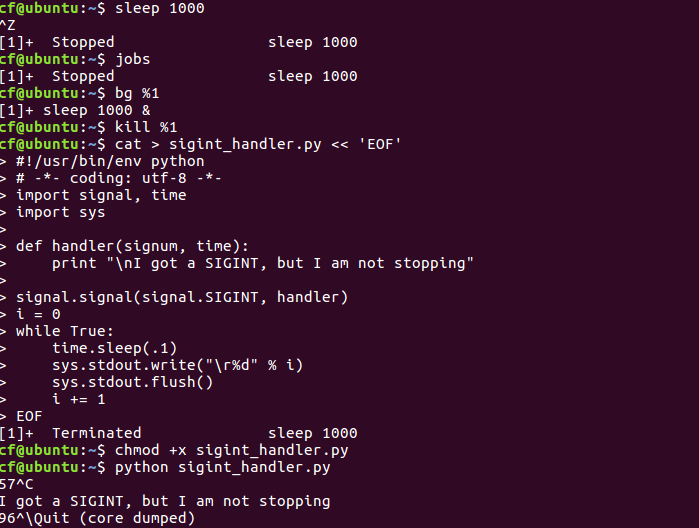
\includegraphics[width=1\textwidth]{image/1.png}
    \caption{实例1}
  \end{figure}
\FloatBarrier
   
  \begin{figure}[htbp]
    \centering
    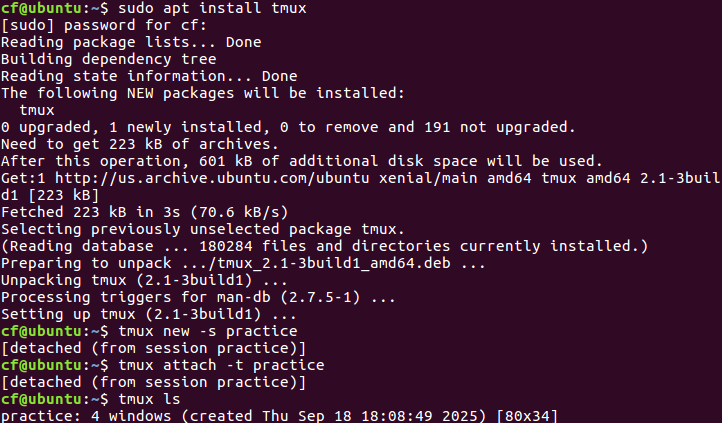
\includegraphics[width=1\textwidth]{image/2.png}
    \caption{实例2}
  \end{figure}
\FloatBarrier
   
    \begin{figure}[htbp]
    \centering
    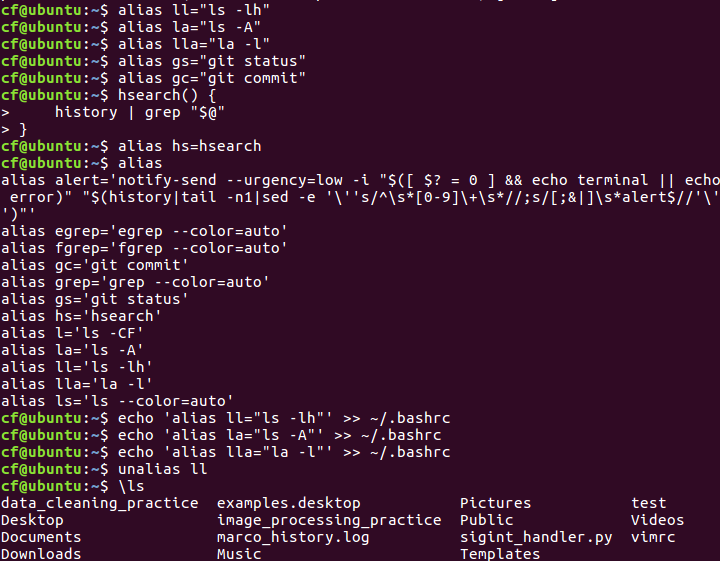
\includegraphics[width=1\textwidth]{image/3.png}
    \caption{实例3}
  \end{figure}
\FloatBarrier
   
    \begin{figure}[htbp]
    \centering
    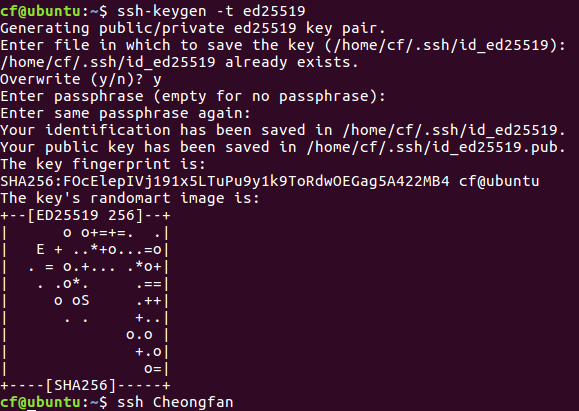
\includegraphics[width=1\textwidth]{image/4.png}
    \caption{实例4}
  \end{figure}
\FloatBarrier
   
    \begin{figure}[htbp]
    \centering
    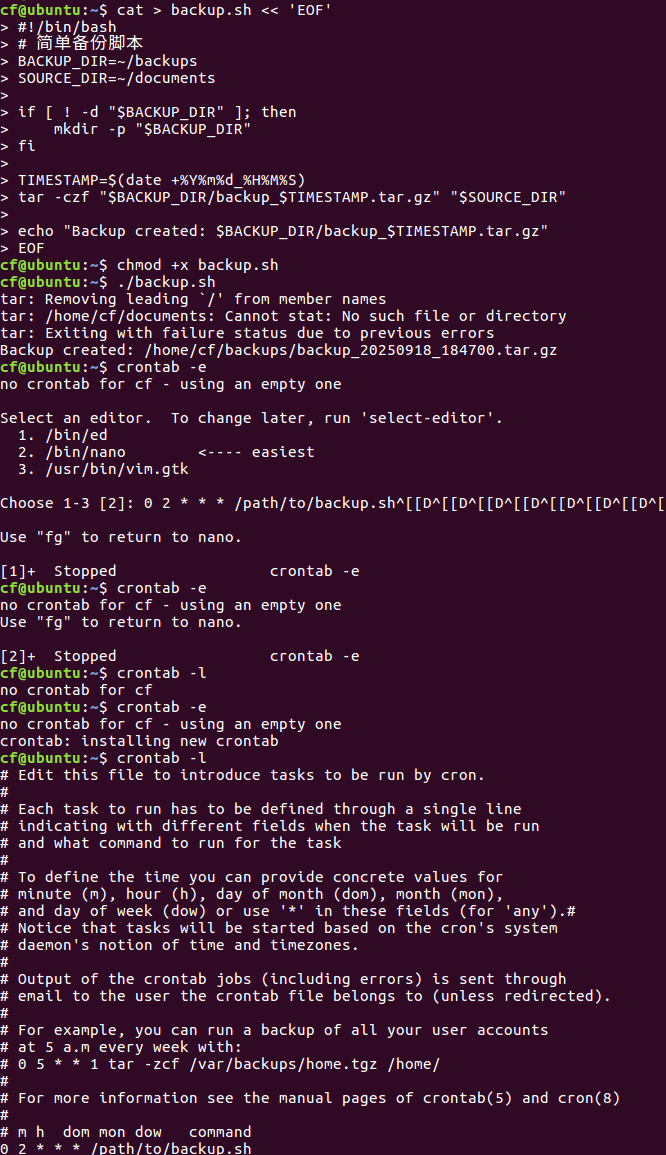
\includegraphics[width=1\textwidth]{image/5.png}
    \caption{实例5}
  \end{figure}
\FloatBarrier
   
    \begin{figure}[htbp]
    \centering
    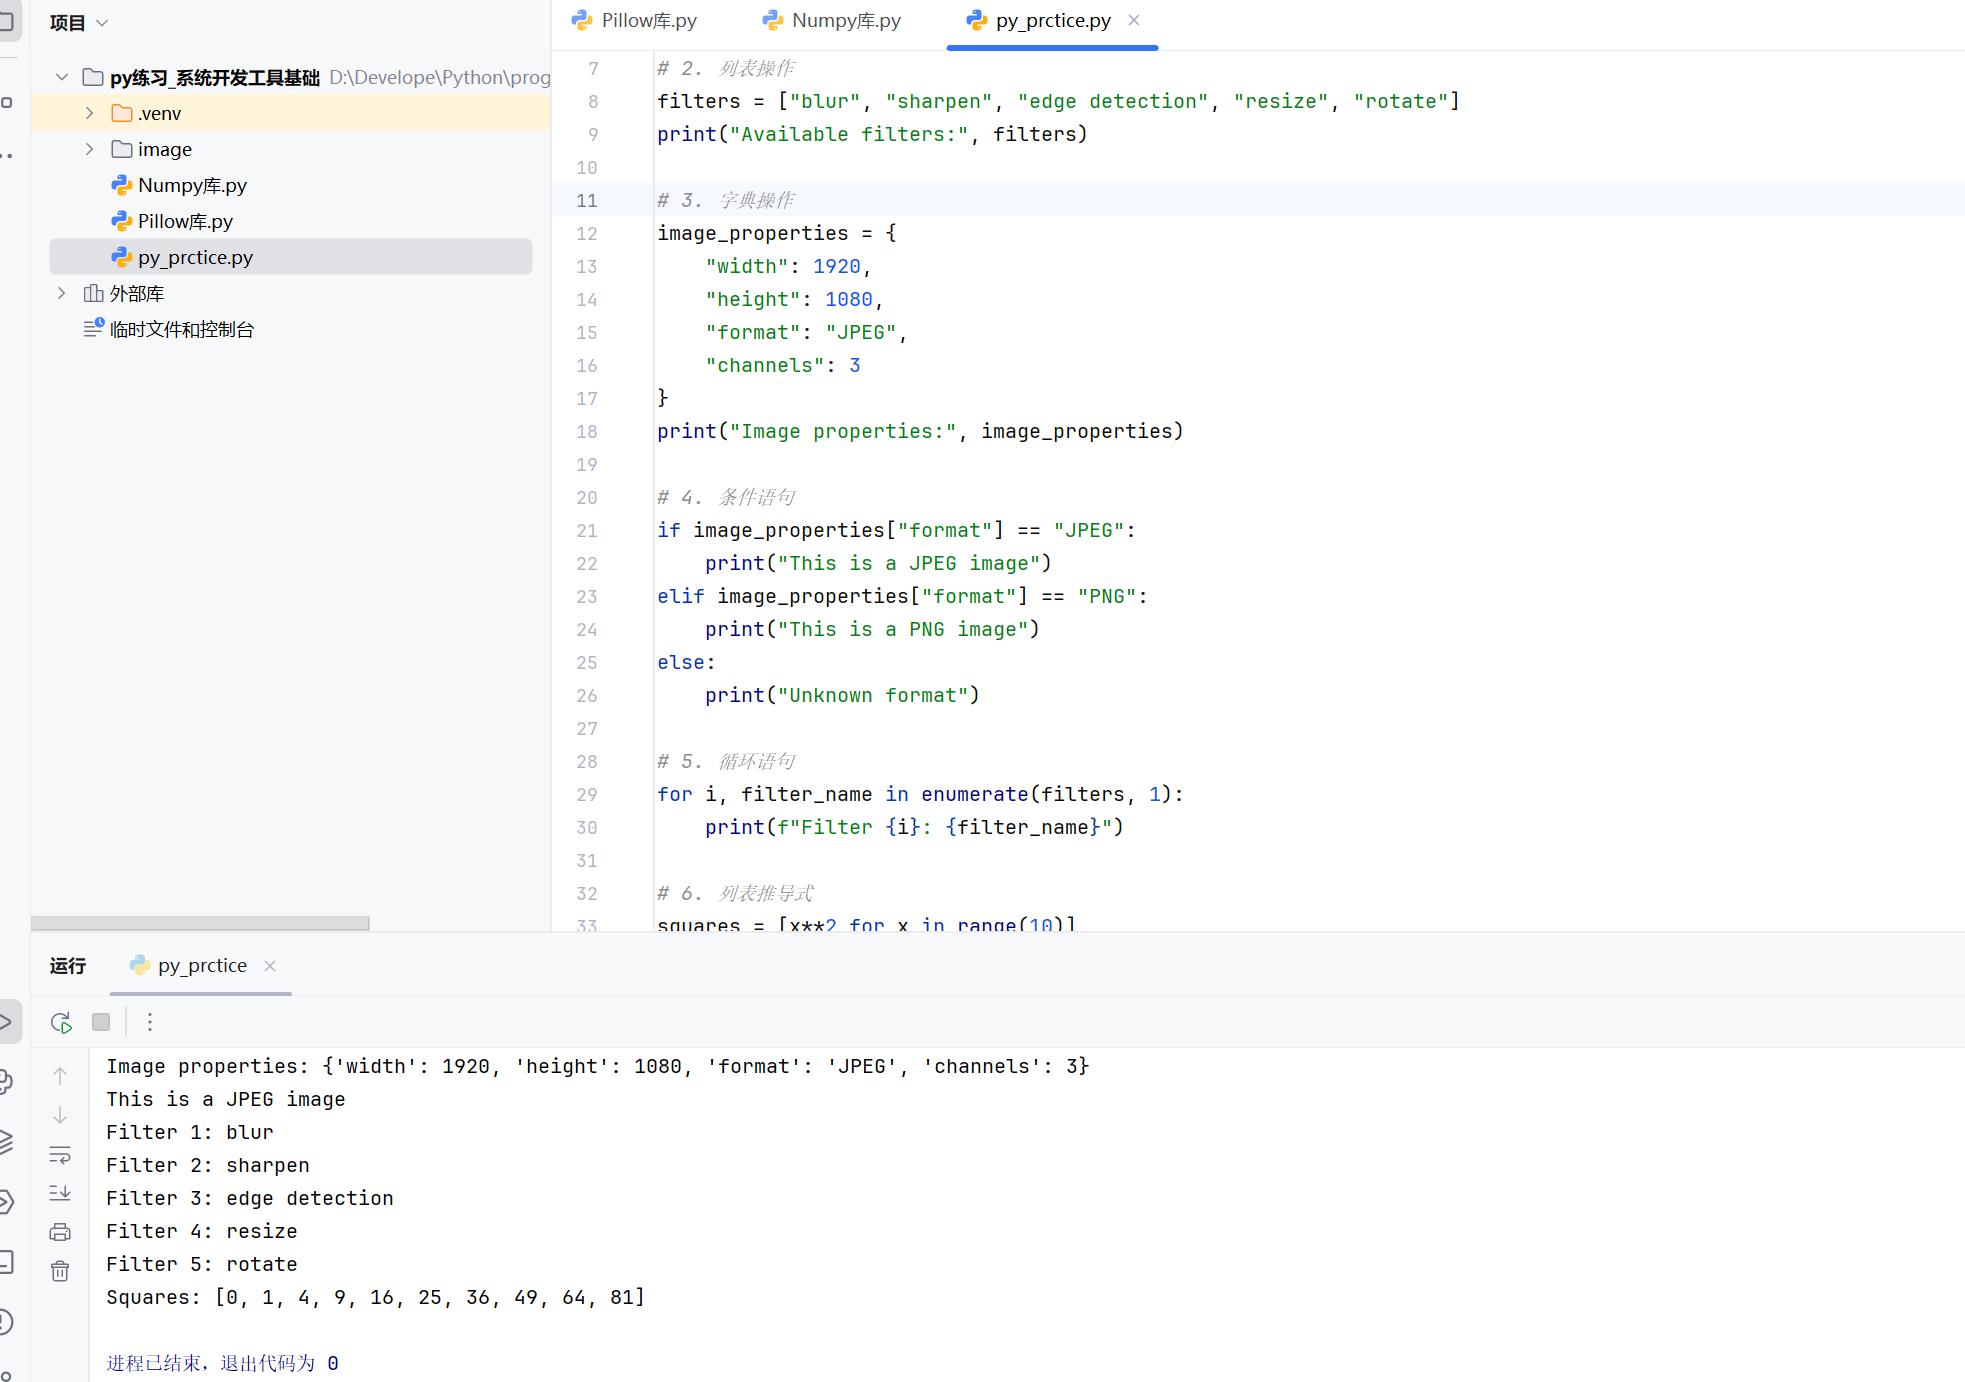
\includegraphics[width=1\textwidth]{image/6.png}
    \caption{实例6}
  \end{figure}
\FloatBarrier
   
    \begin{figure}[htbp]
    \centering
    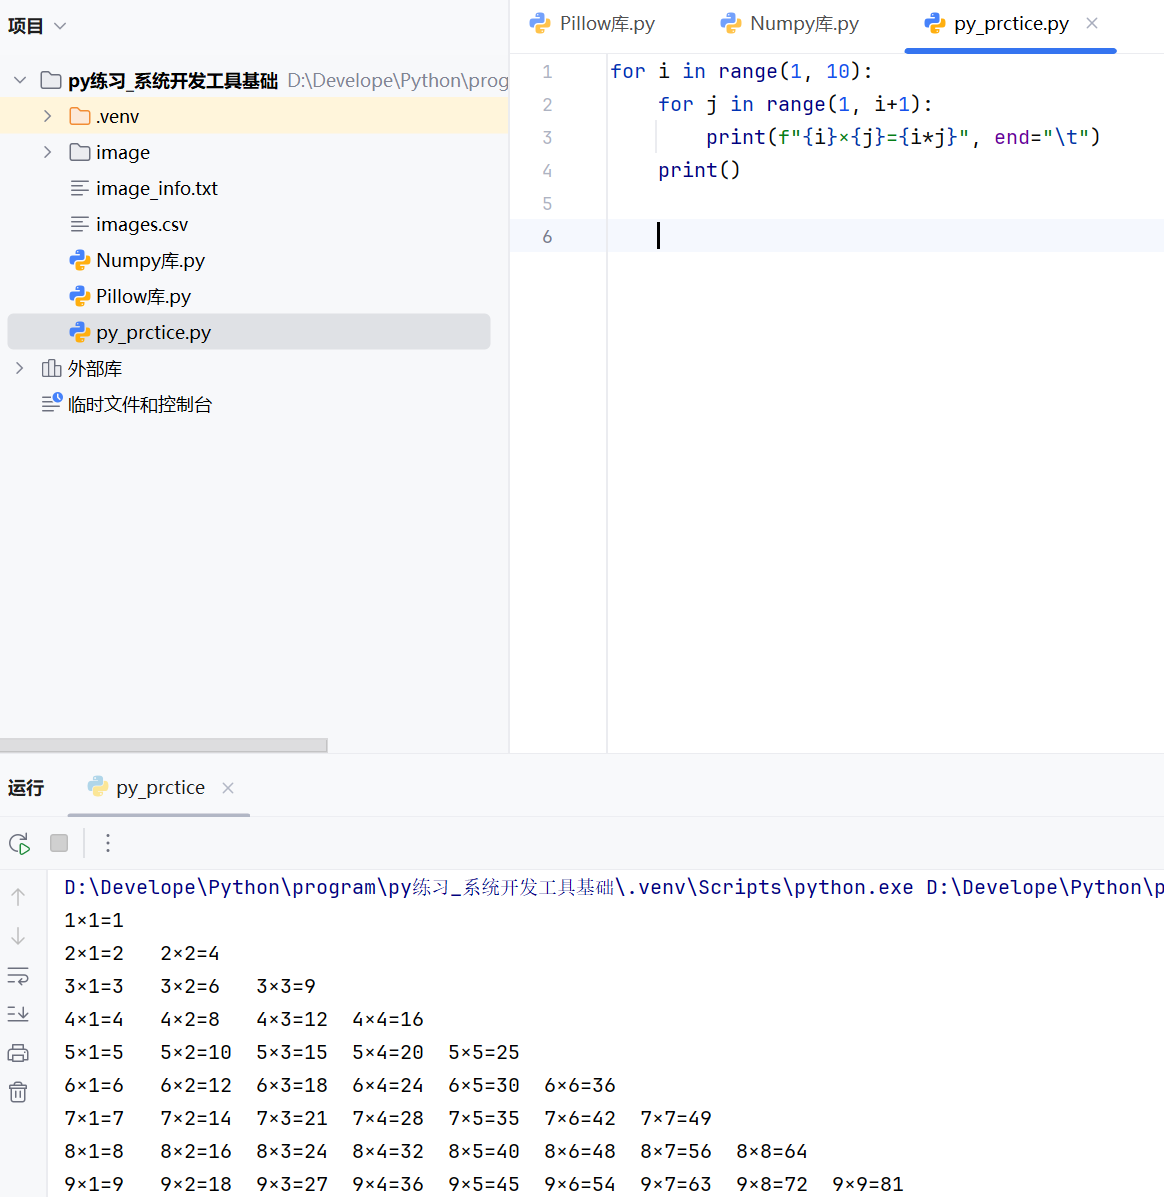
\includegraphics[width=1\textwidth]{image/13.png}
    \caption{实例7}
  \end{figure}
\FloatBarrier
   
    \begin{figure}[htbp]
    \centering
    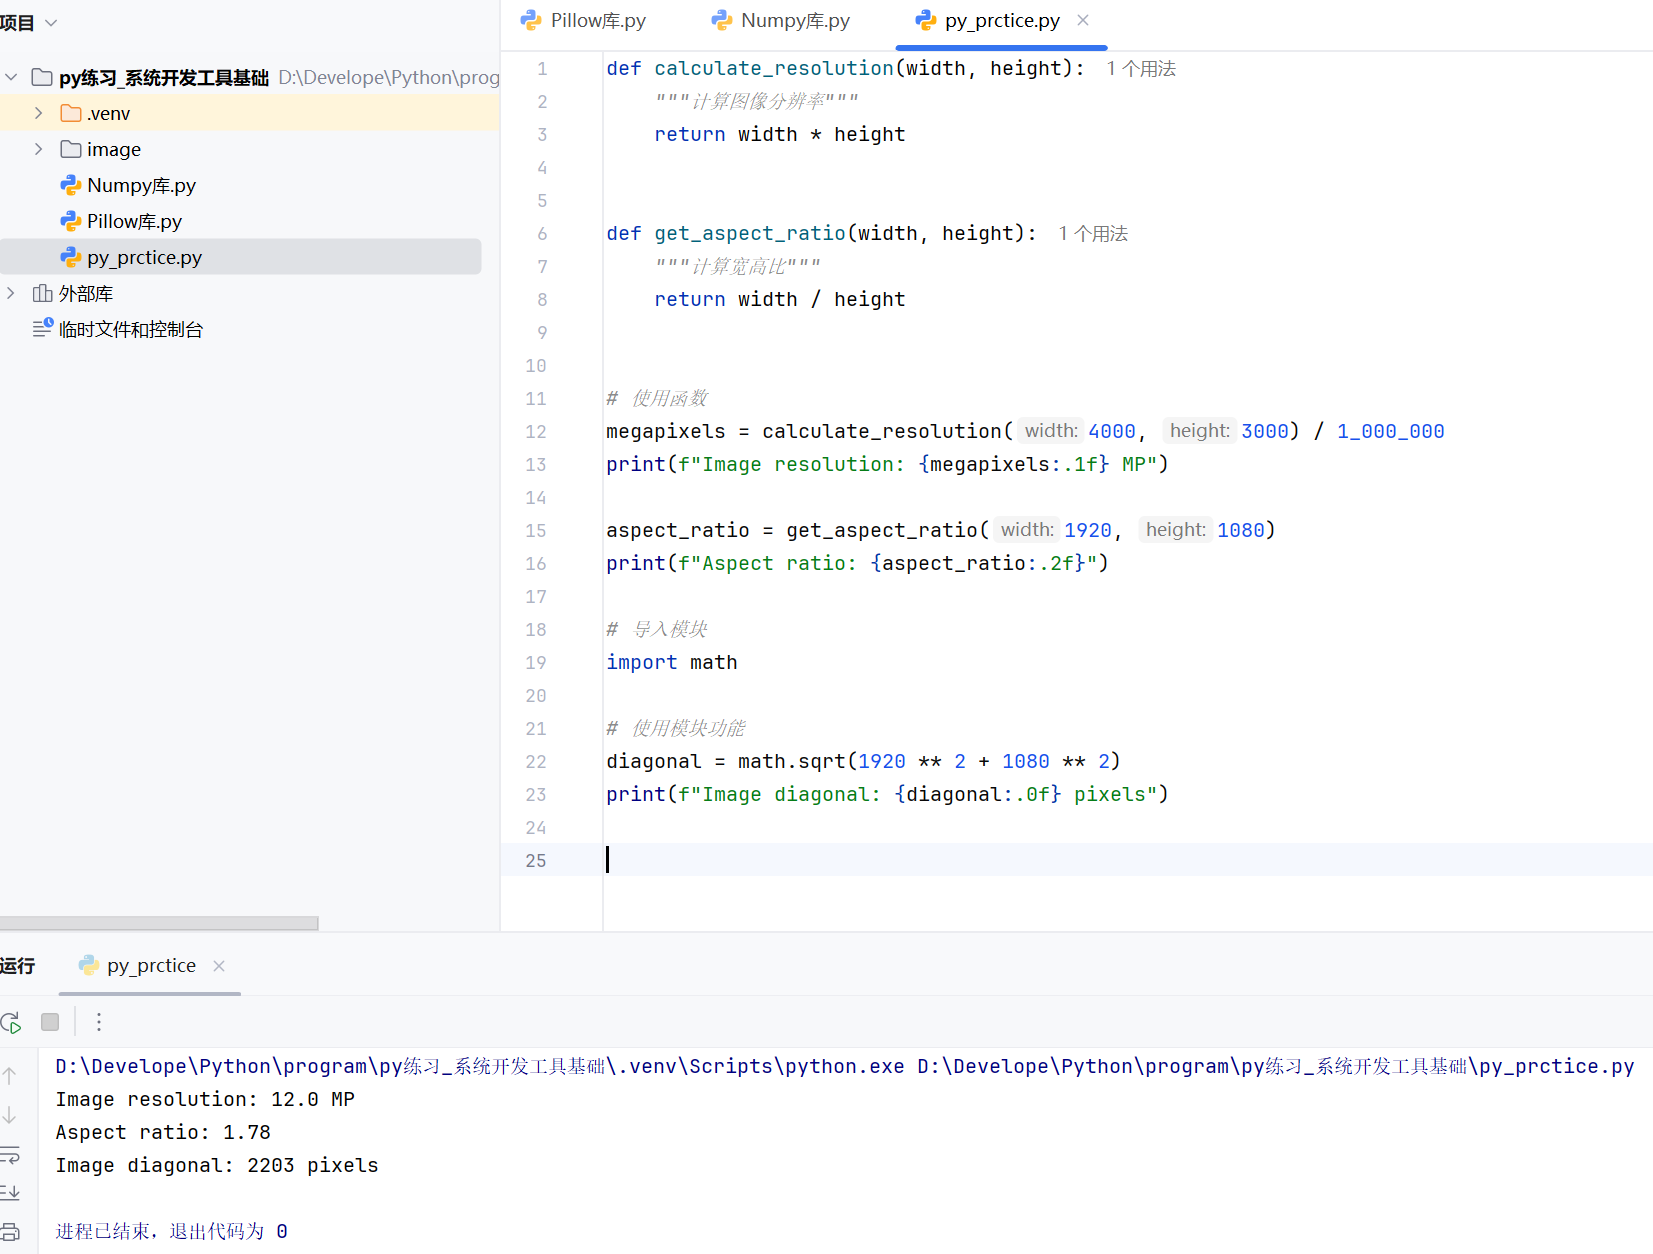
\includegraphics[width=1\textwidth]{image/7.png}
    \caption{实例8}
  \end{figure}
\FloatBarrier
   
      \begin{figure}[htbp]
    \centering
    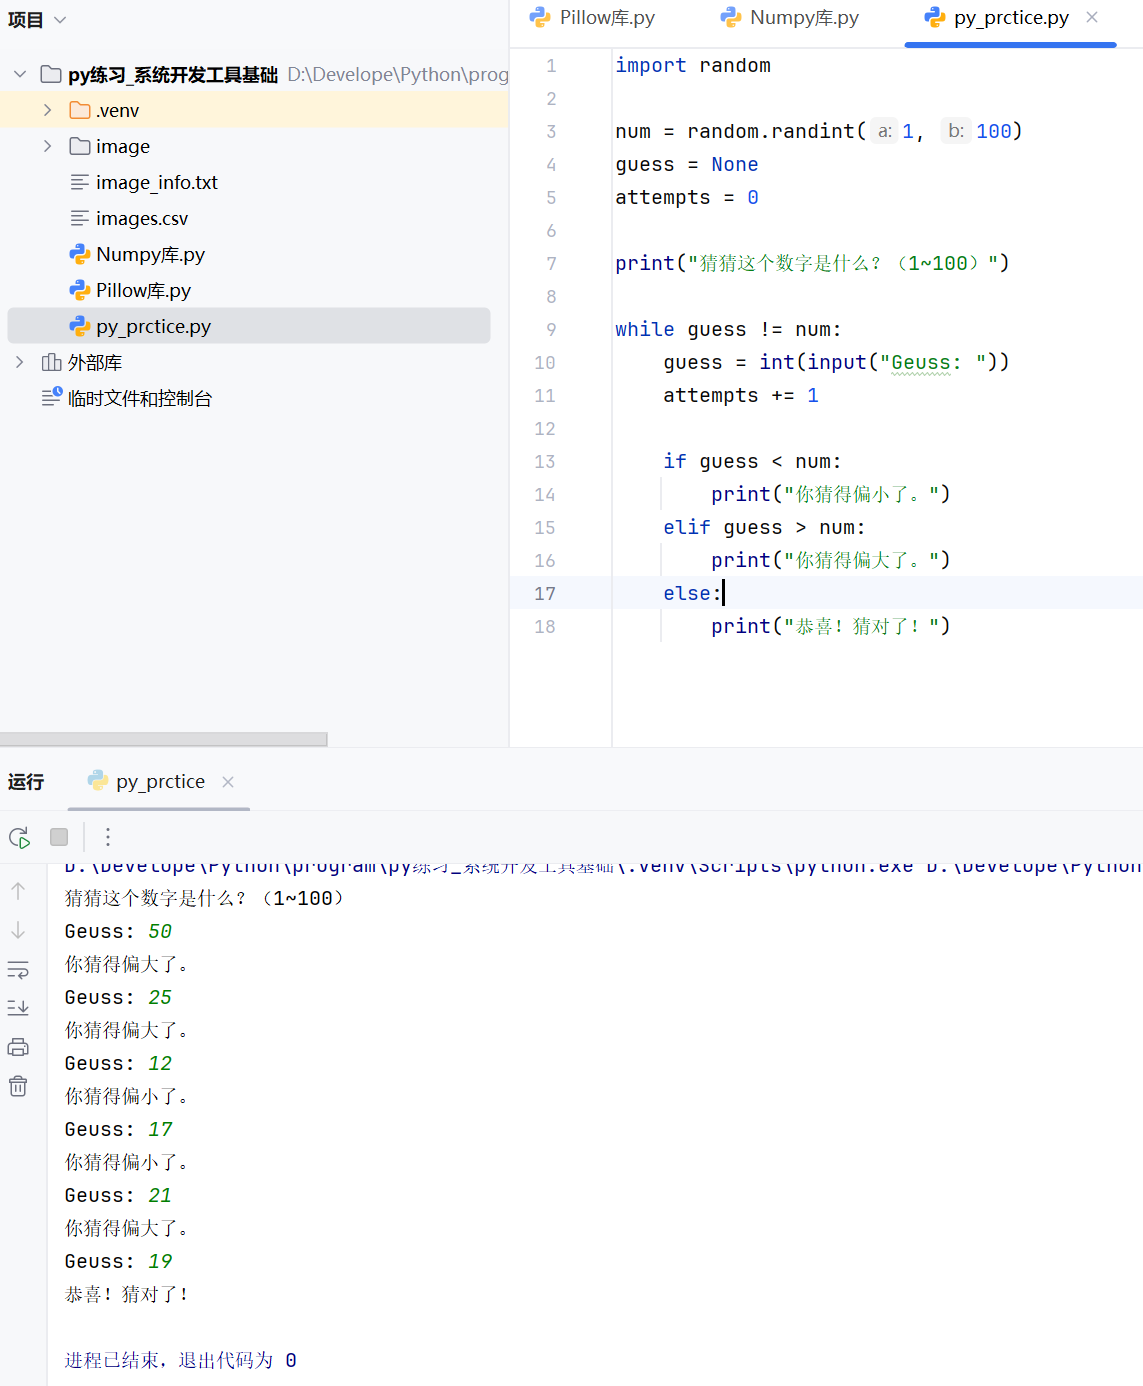
\includegraphics[width=1\textwidth]{image/12.png}
    \caption{实例9}
  \end{figure}
\FloatBarrier
   
      \begin{figure}[htbp]
    \centering
    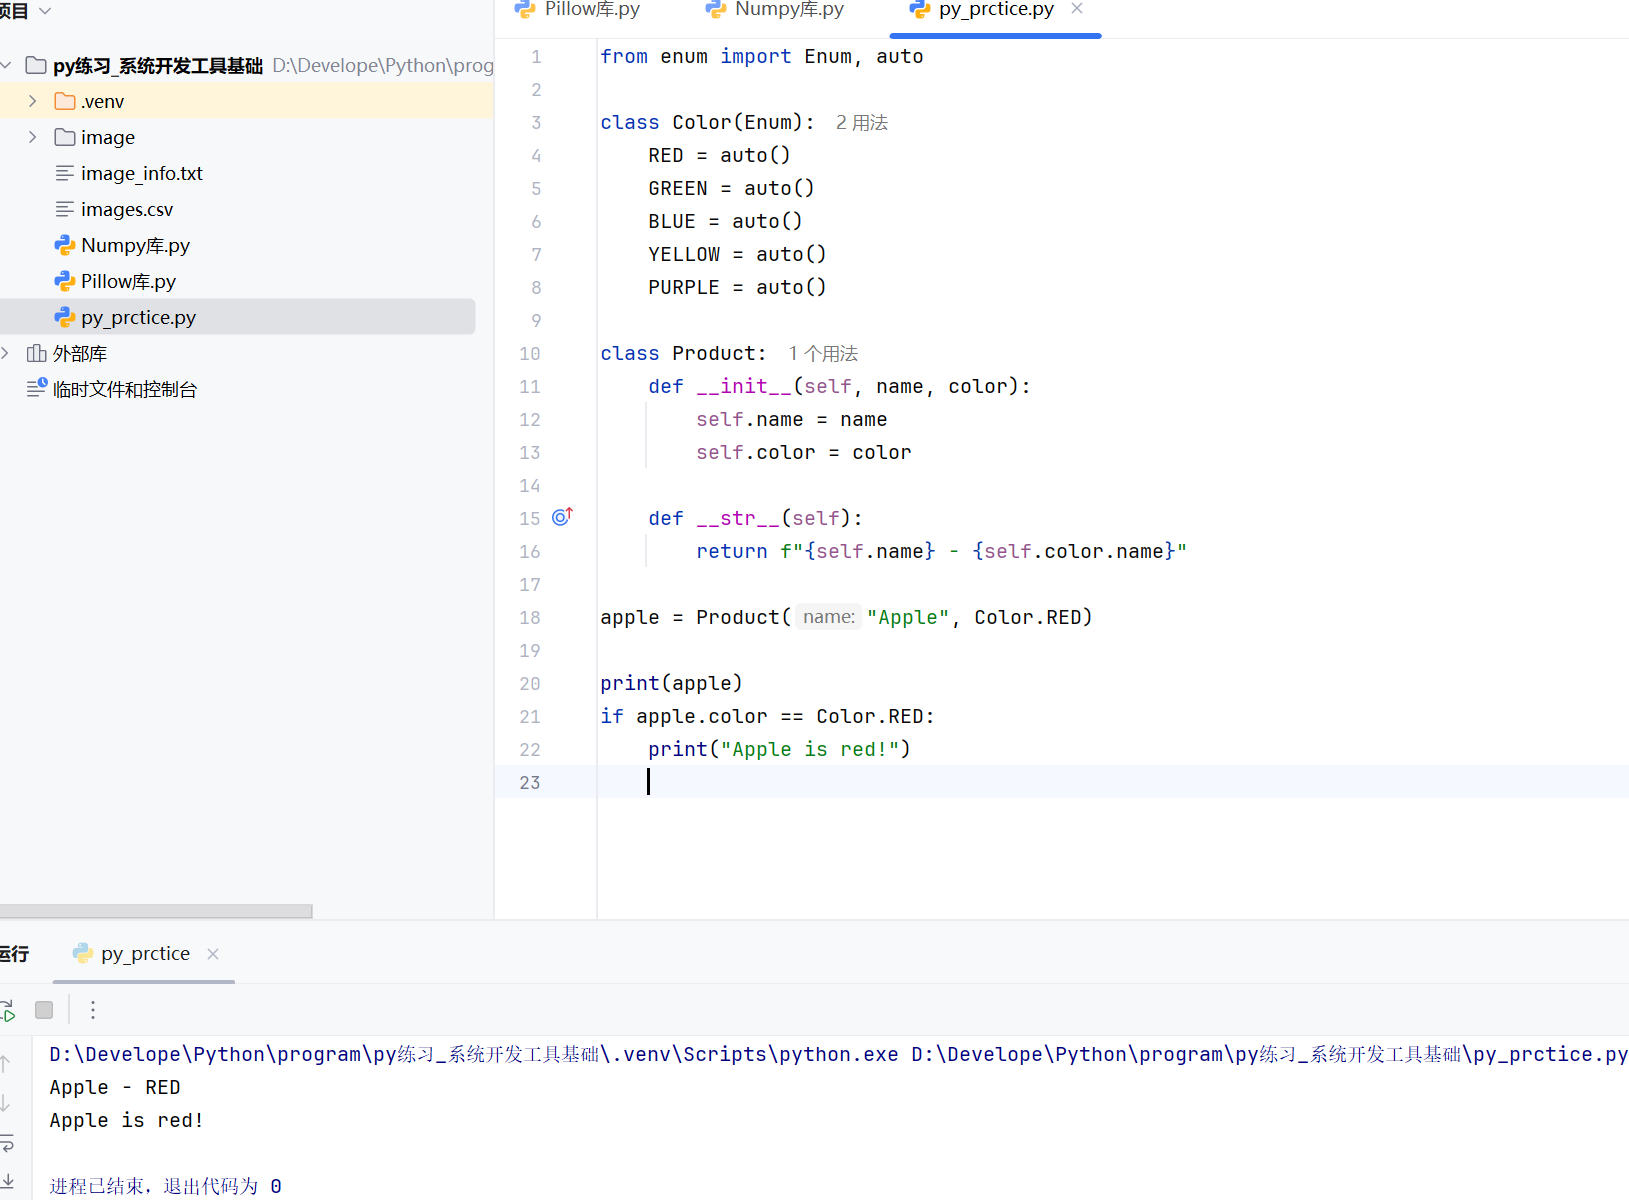
\includegraphics[width=1\textwidth]{image/11.png}
    \caption{实例10}
  \end{figure}
\FloatBarrier
   
      \begin{figure}[htbp]
    \centering
    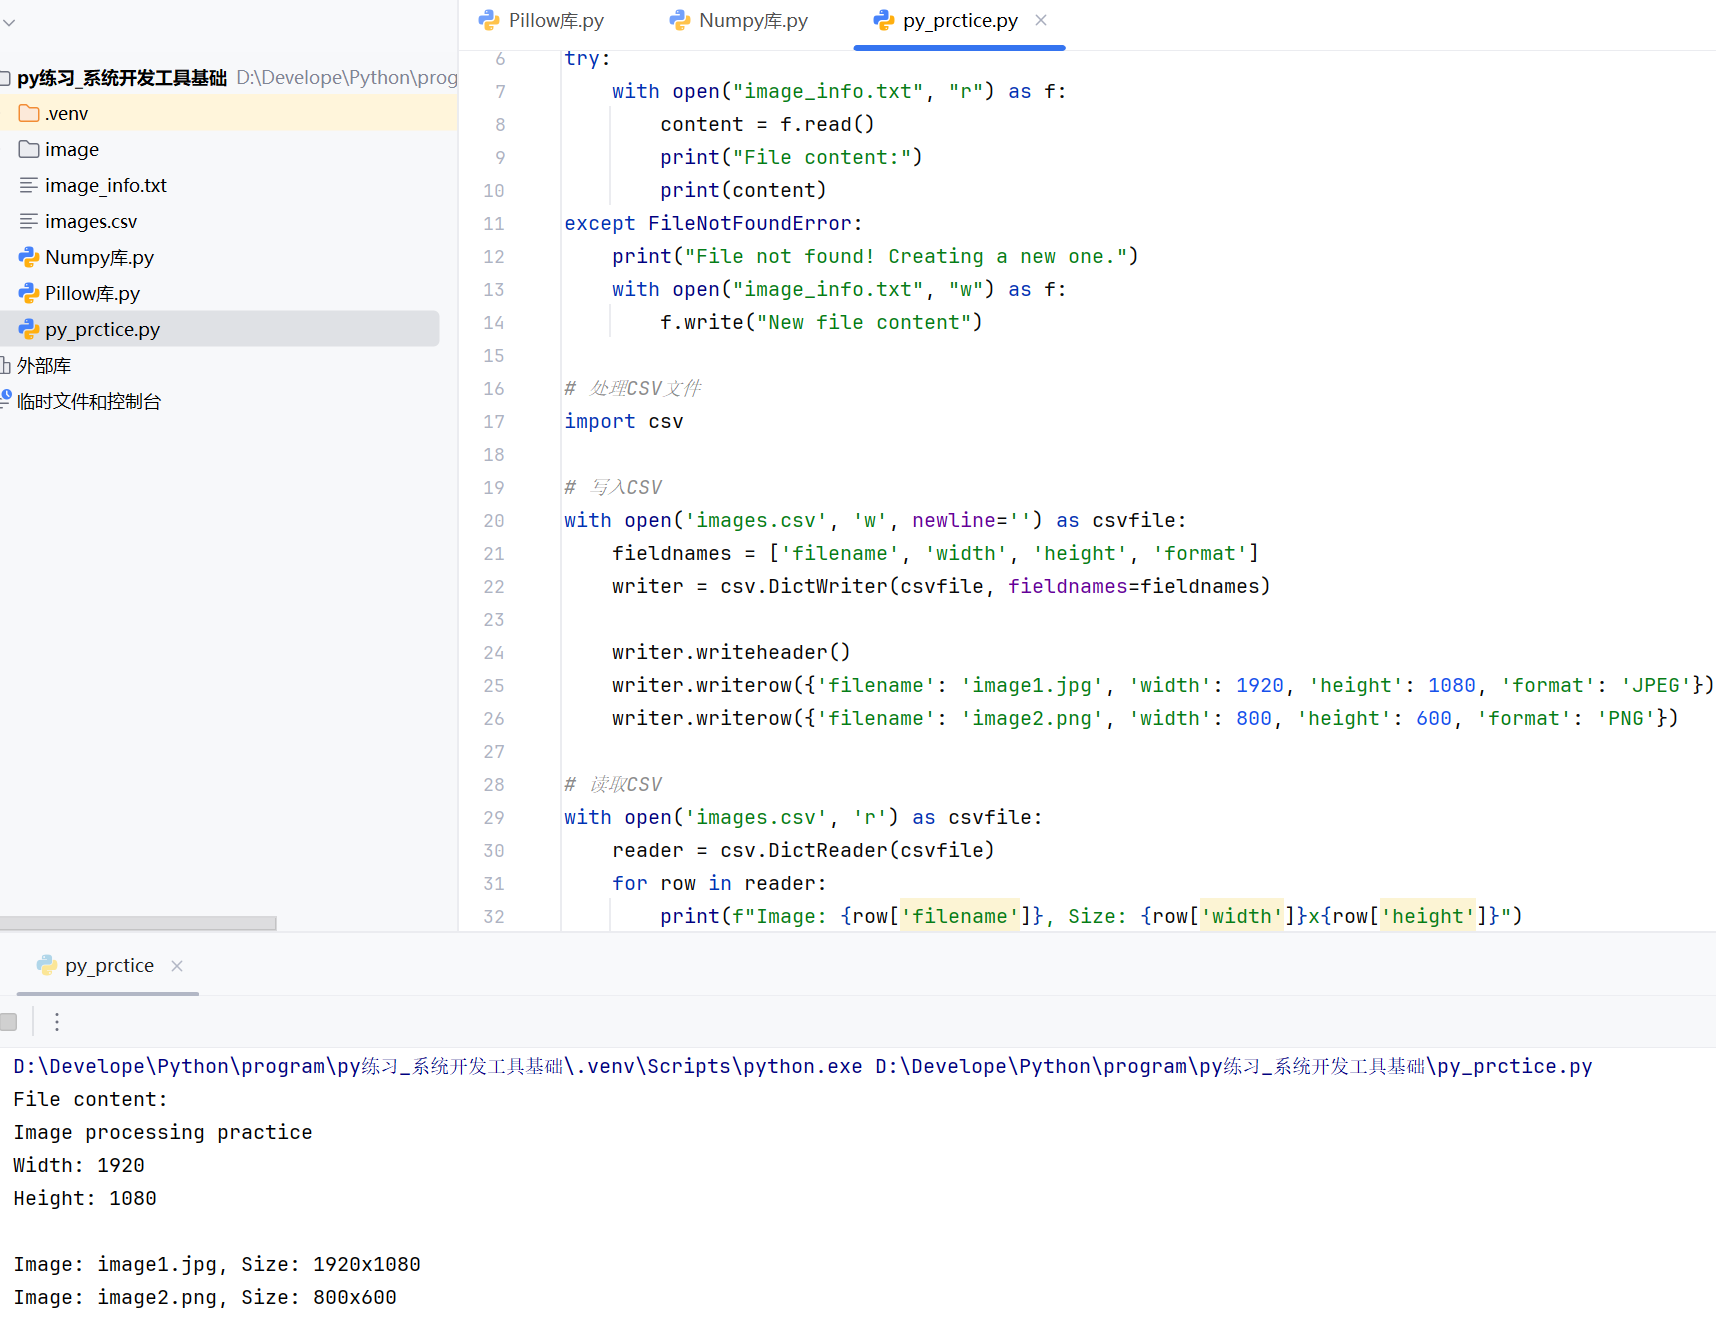
\includegraphics[width=1\textwidth]{image/8.png}
    \caption{实例11}
  \end{figure}
\FloatBarrier
   
      \begin{figure}[htbp]
    \centering
    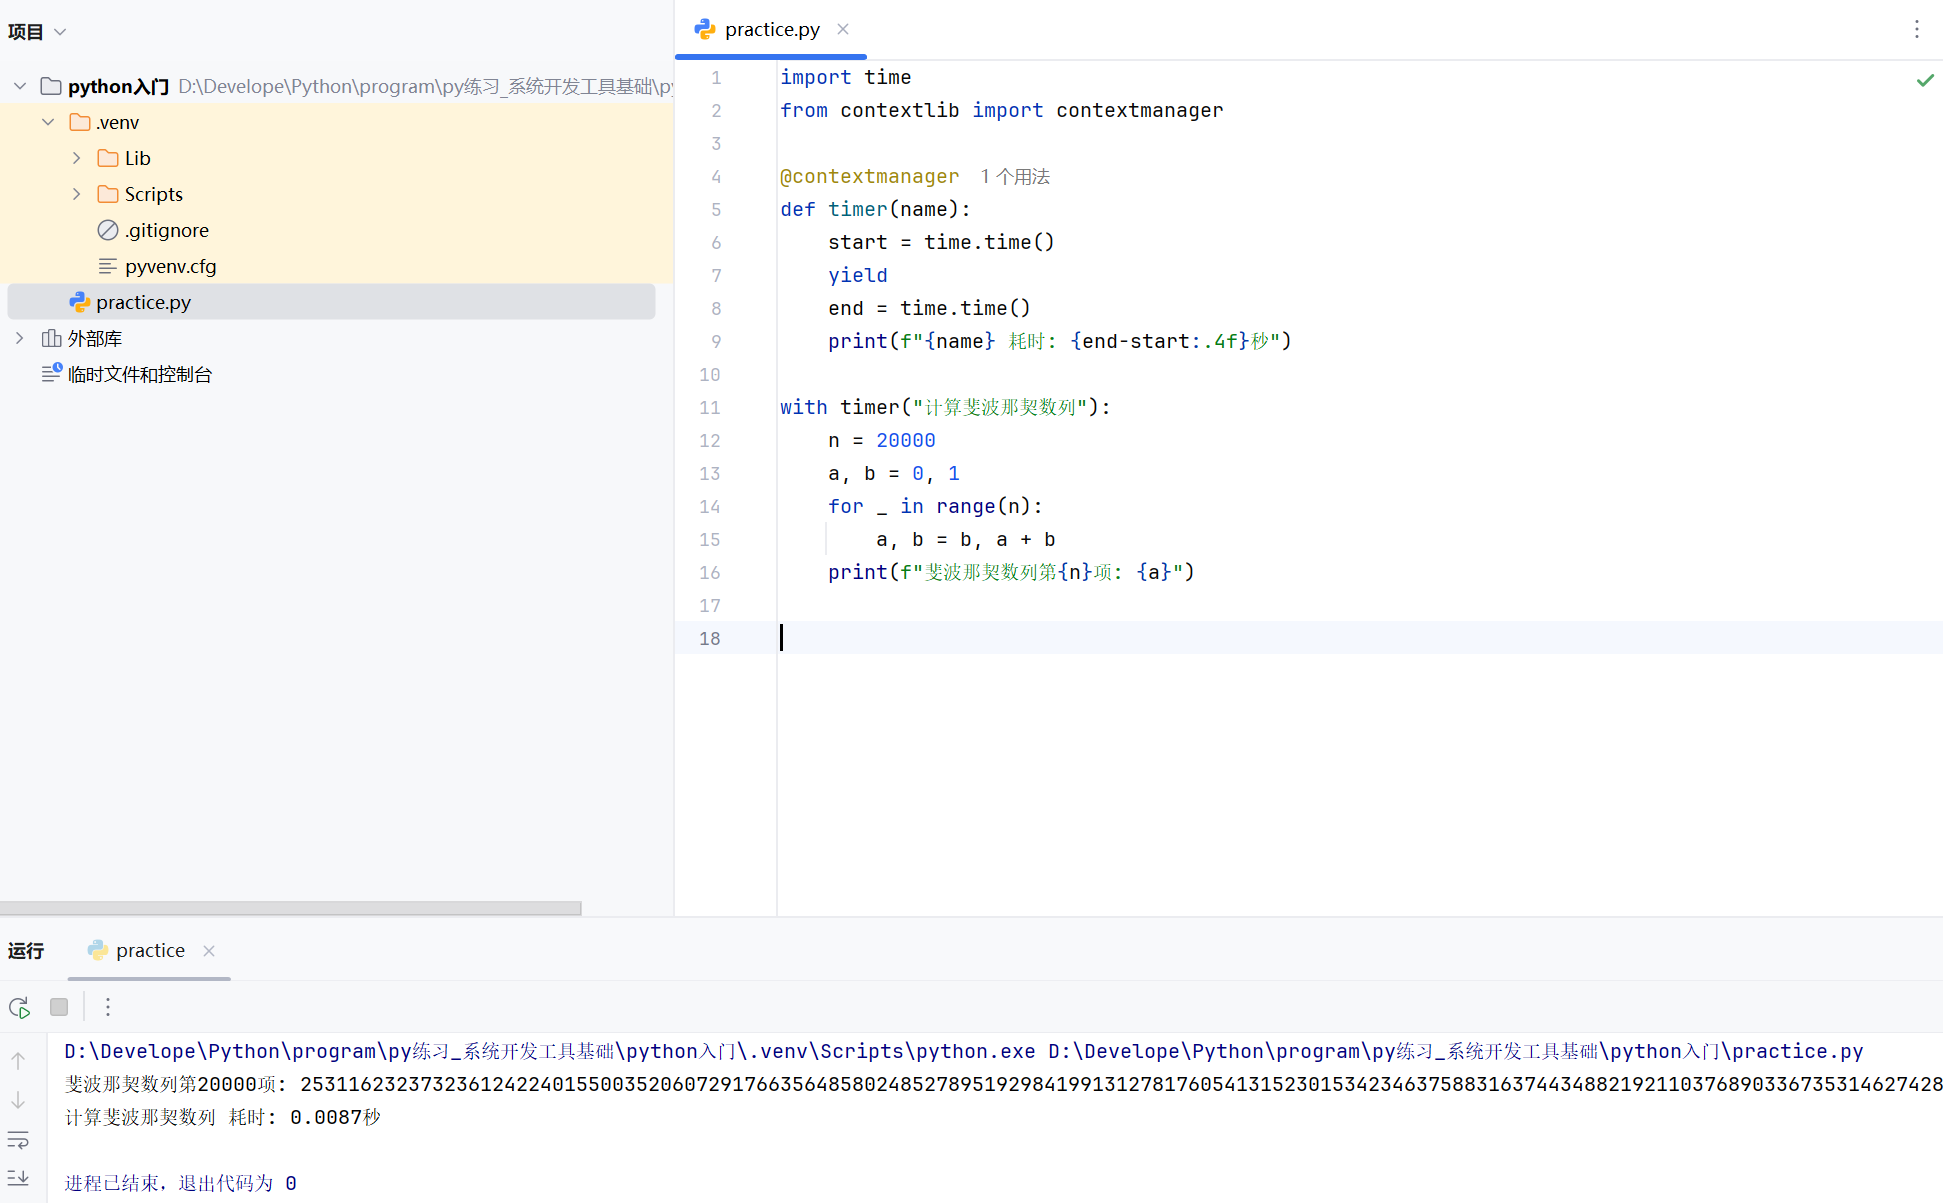
\includegraphics[width=1\textwidth]{image/20.png}
    \caption{实例12}
  \end{figure}
\FloatBarrier
   
      \begin{figure}[htbp]
    \centering
    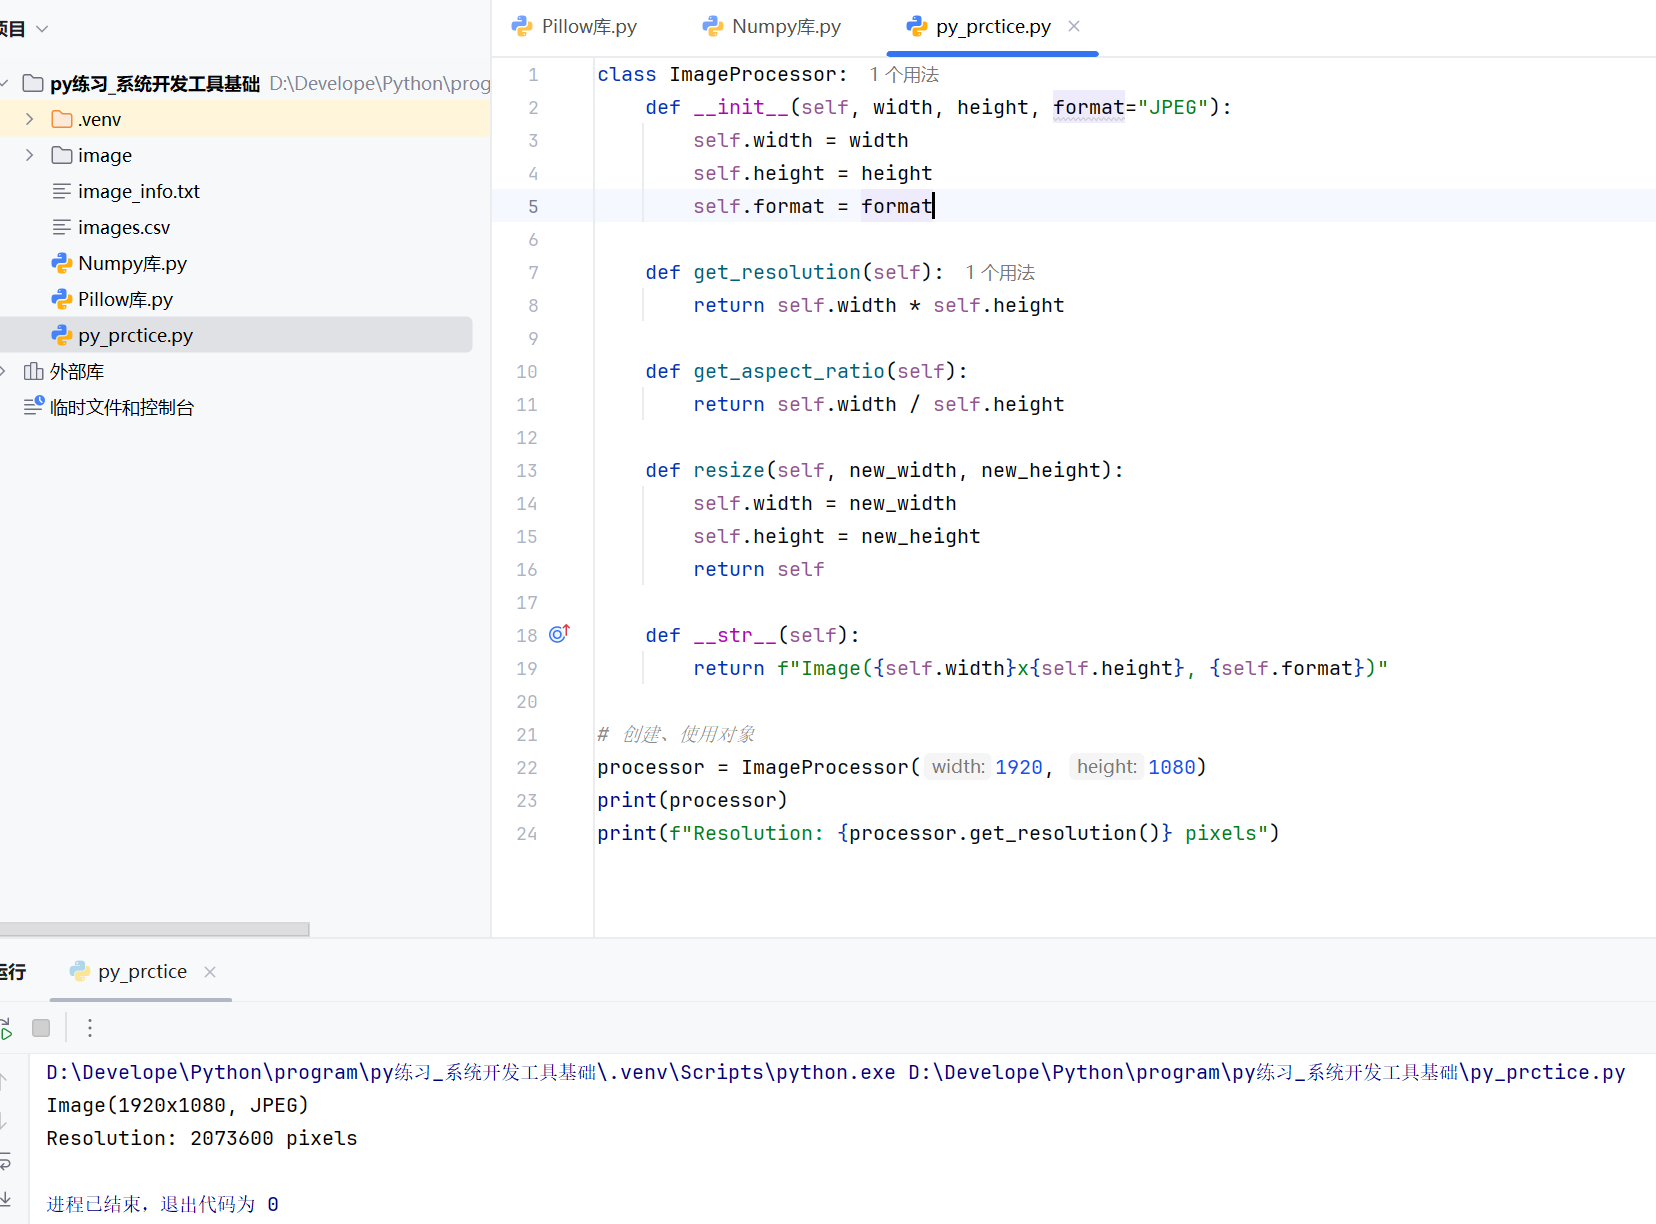
\includegraphics[width=1\textwidth]{image/9.png}
    \caption{实例13}
  \end{figure}
\FloatBarrier
   
    \begin{figure}[htbp]
    \centering
    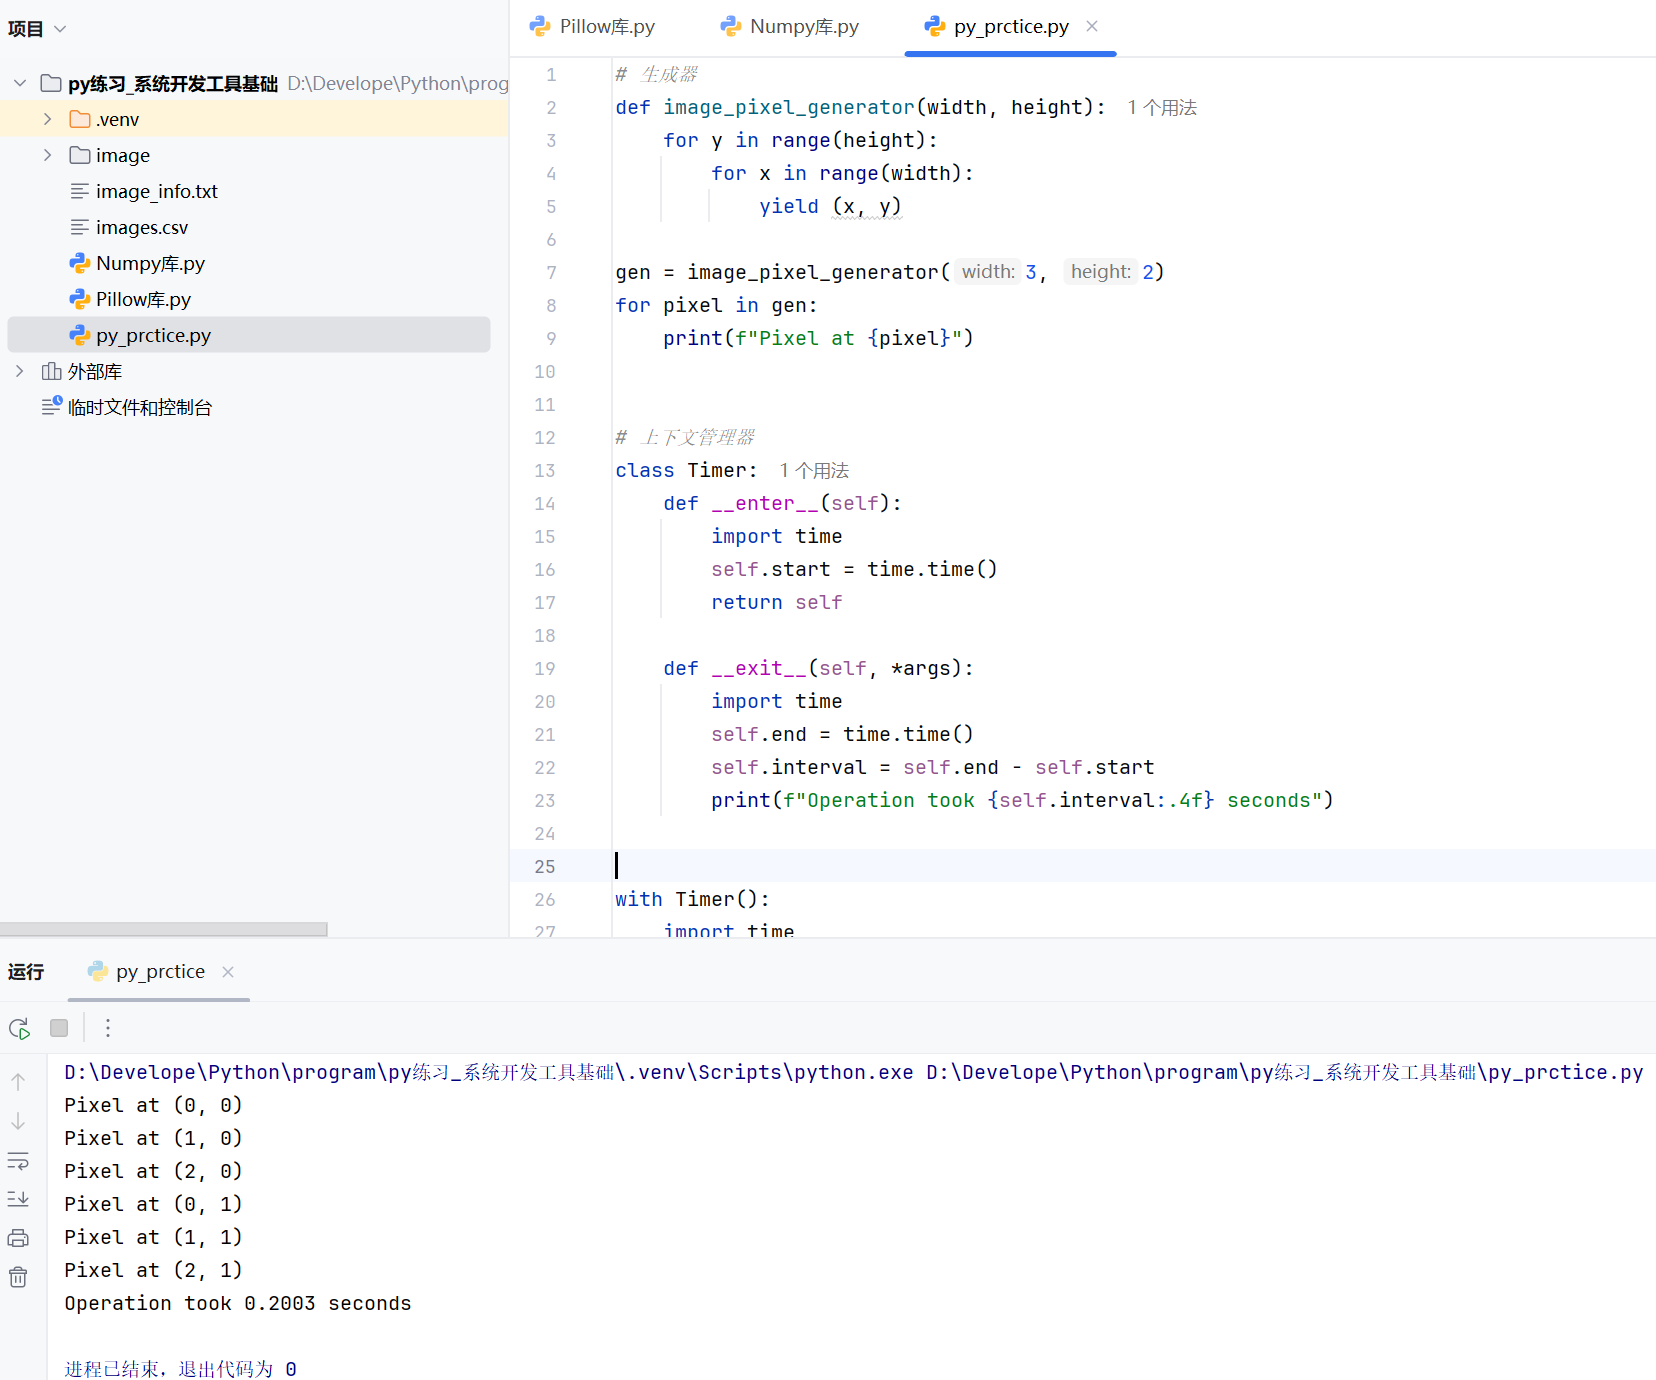
\includegraphics[width=1\textwidth]{image/10.png}
    \caption{实例14}
  \end{figure}
\FloatBarrier
   
    \begin{figure}[htbp]
    \centering
    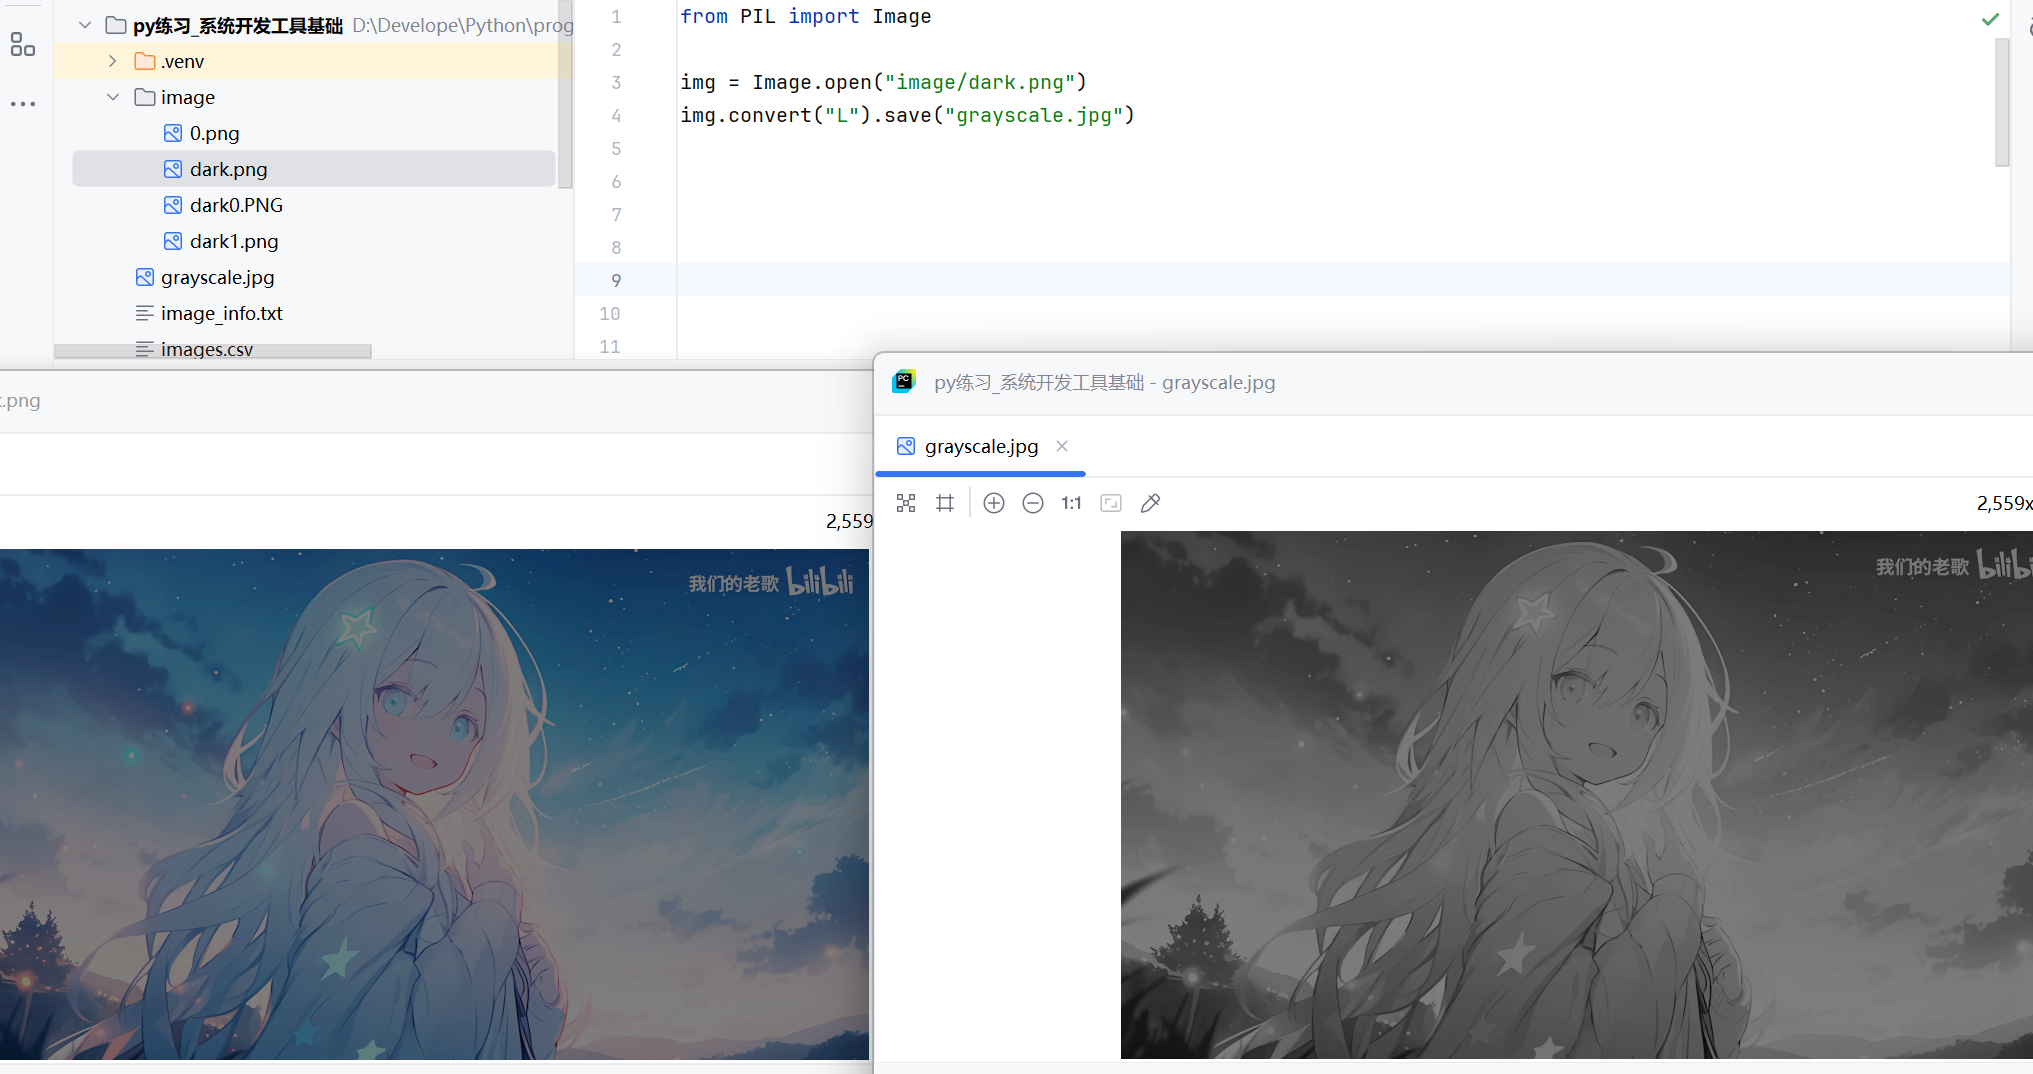
\includegraphics[width=1\textwidth]{image/14.png}
    \caption{实例15}
  \end{figure}
\FloatBarrier
   
      \begin{figure}[htbp]
    \centering
    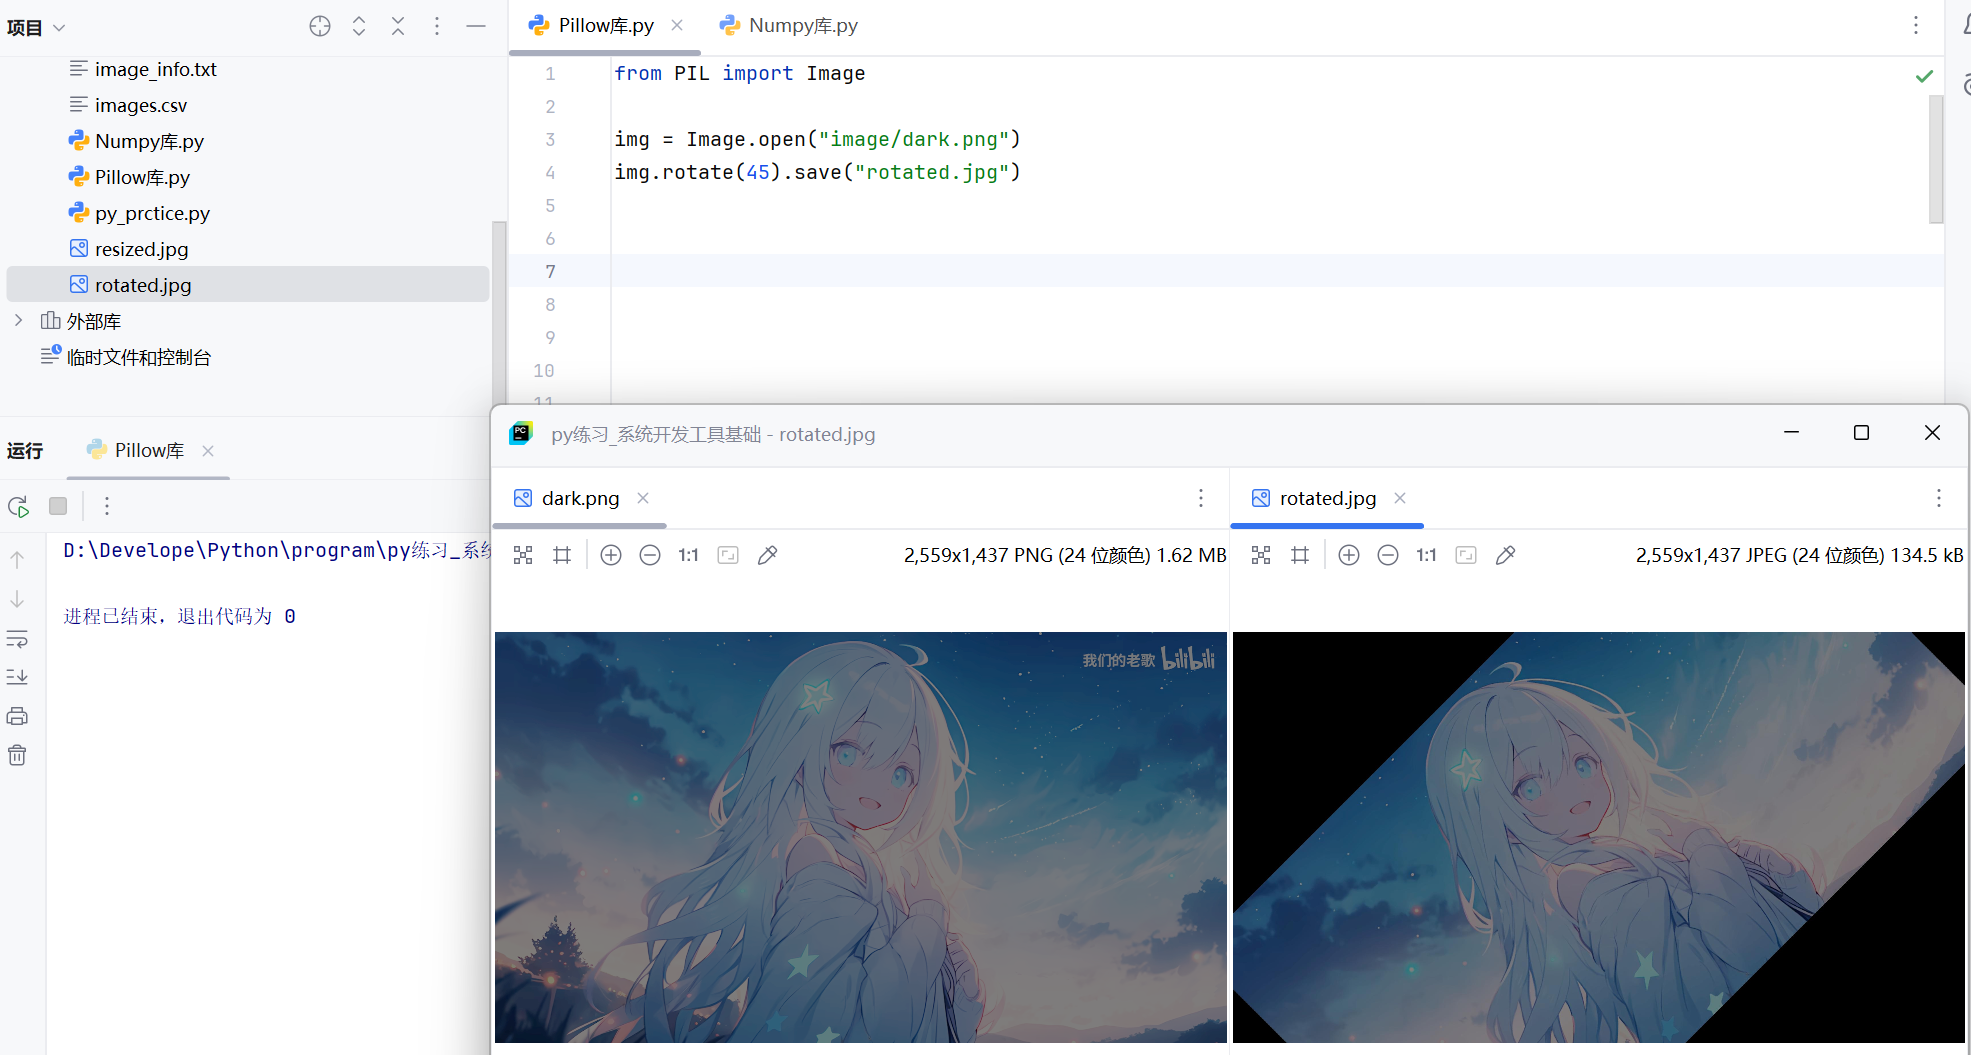
\includegraphics[width=1\textwidth]{image/15.png}
    \caption{实例16}
  \end{figure}
\FloatBarrier
   
      \begin{figure}[htbp]
    \centering
    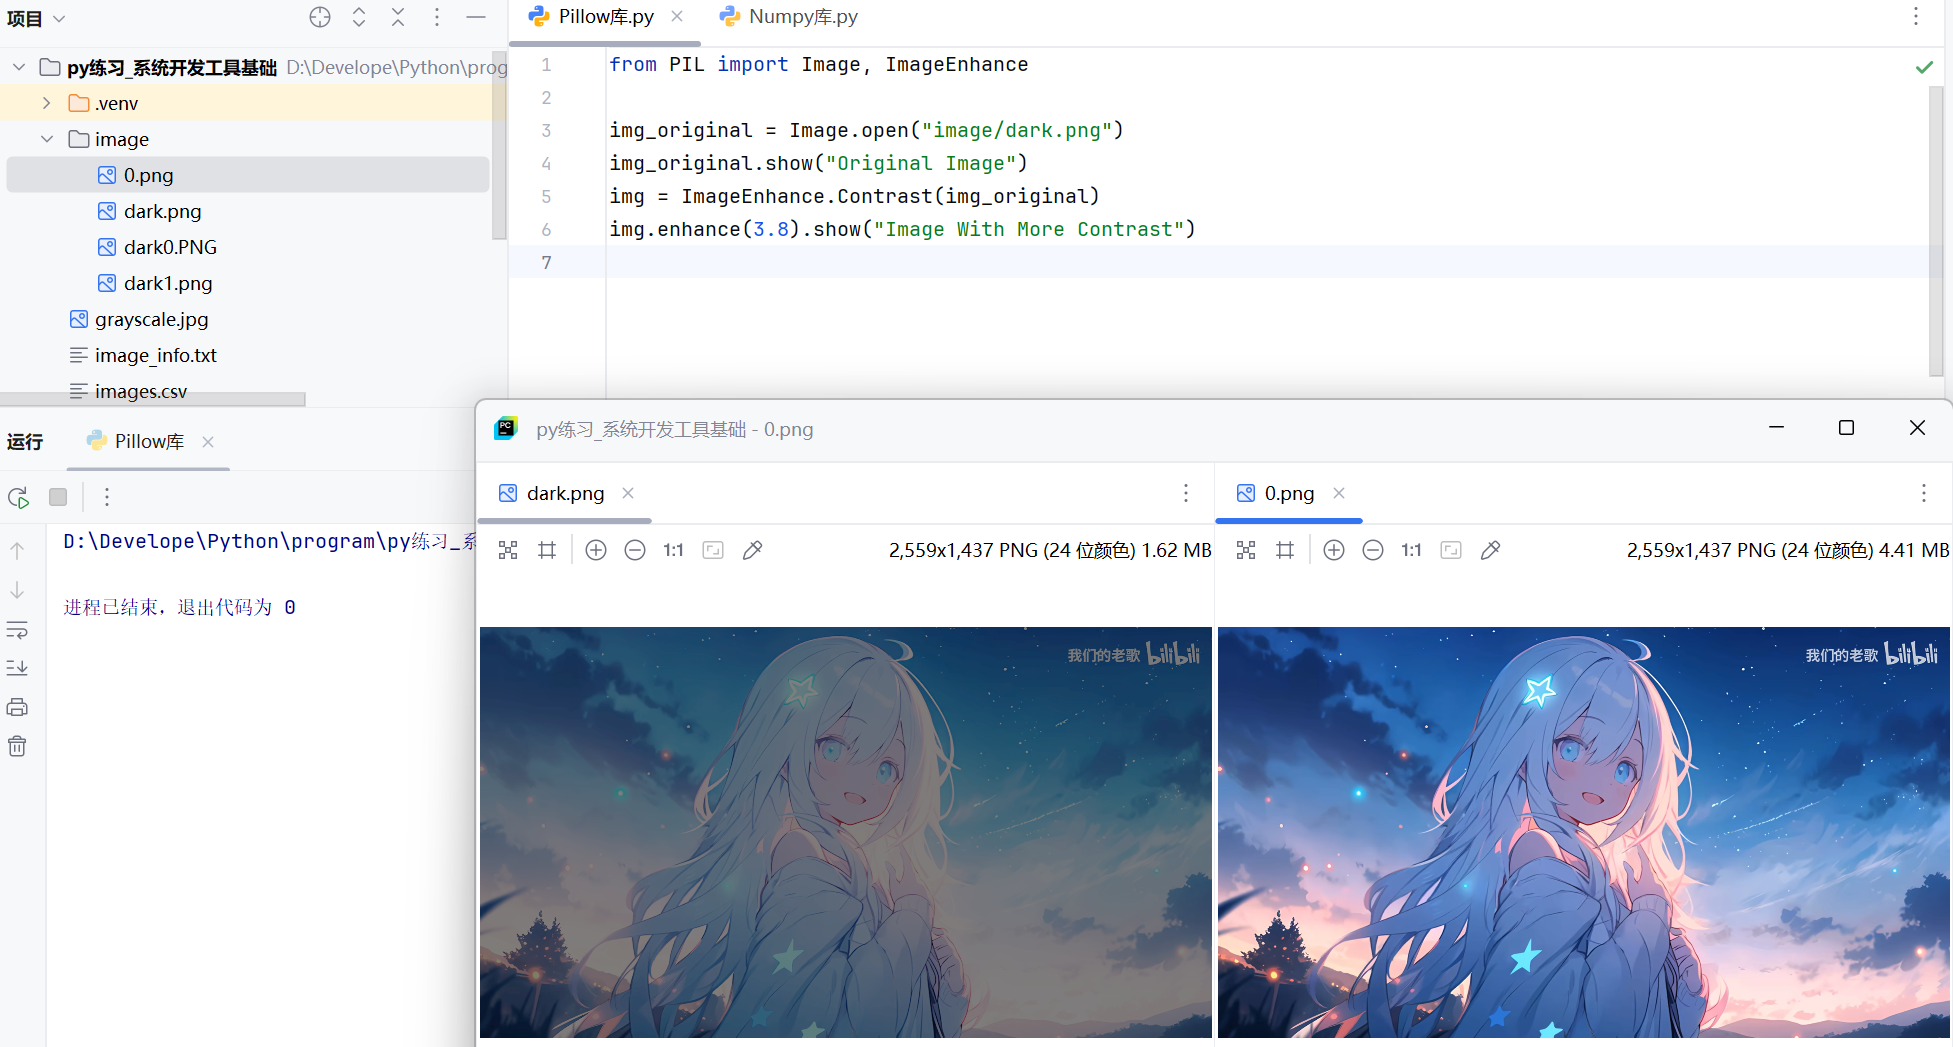
\includegraphics[width=1\textwidth]{image/16.png}
    \caption{实例17}
  \end{figure}
\FloatBarrier
    \begin{figure}[htbp]
    \centering
    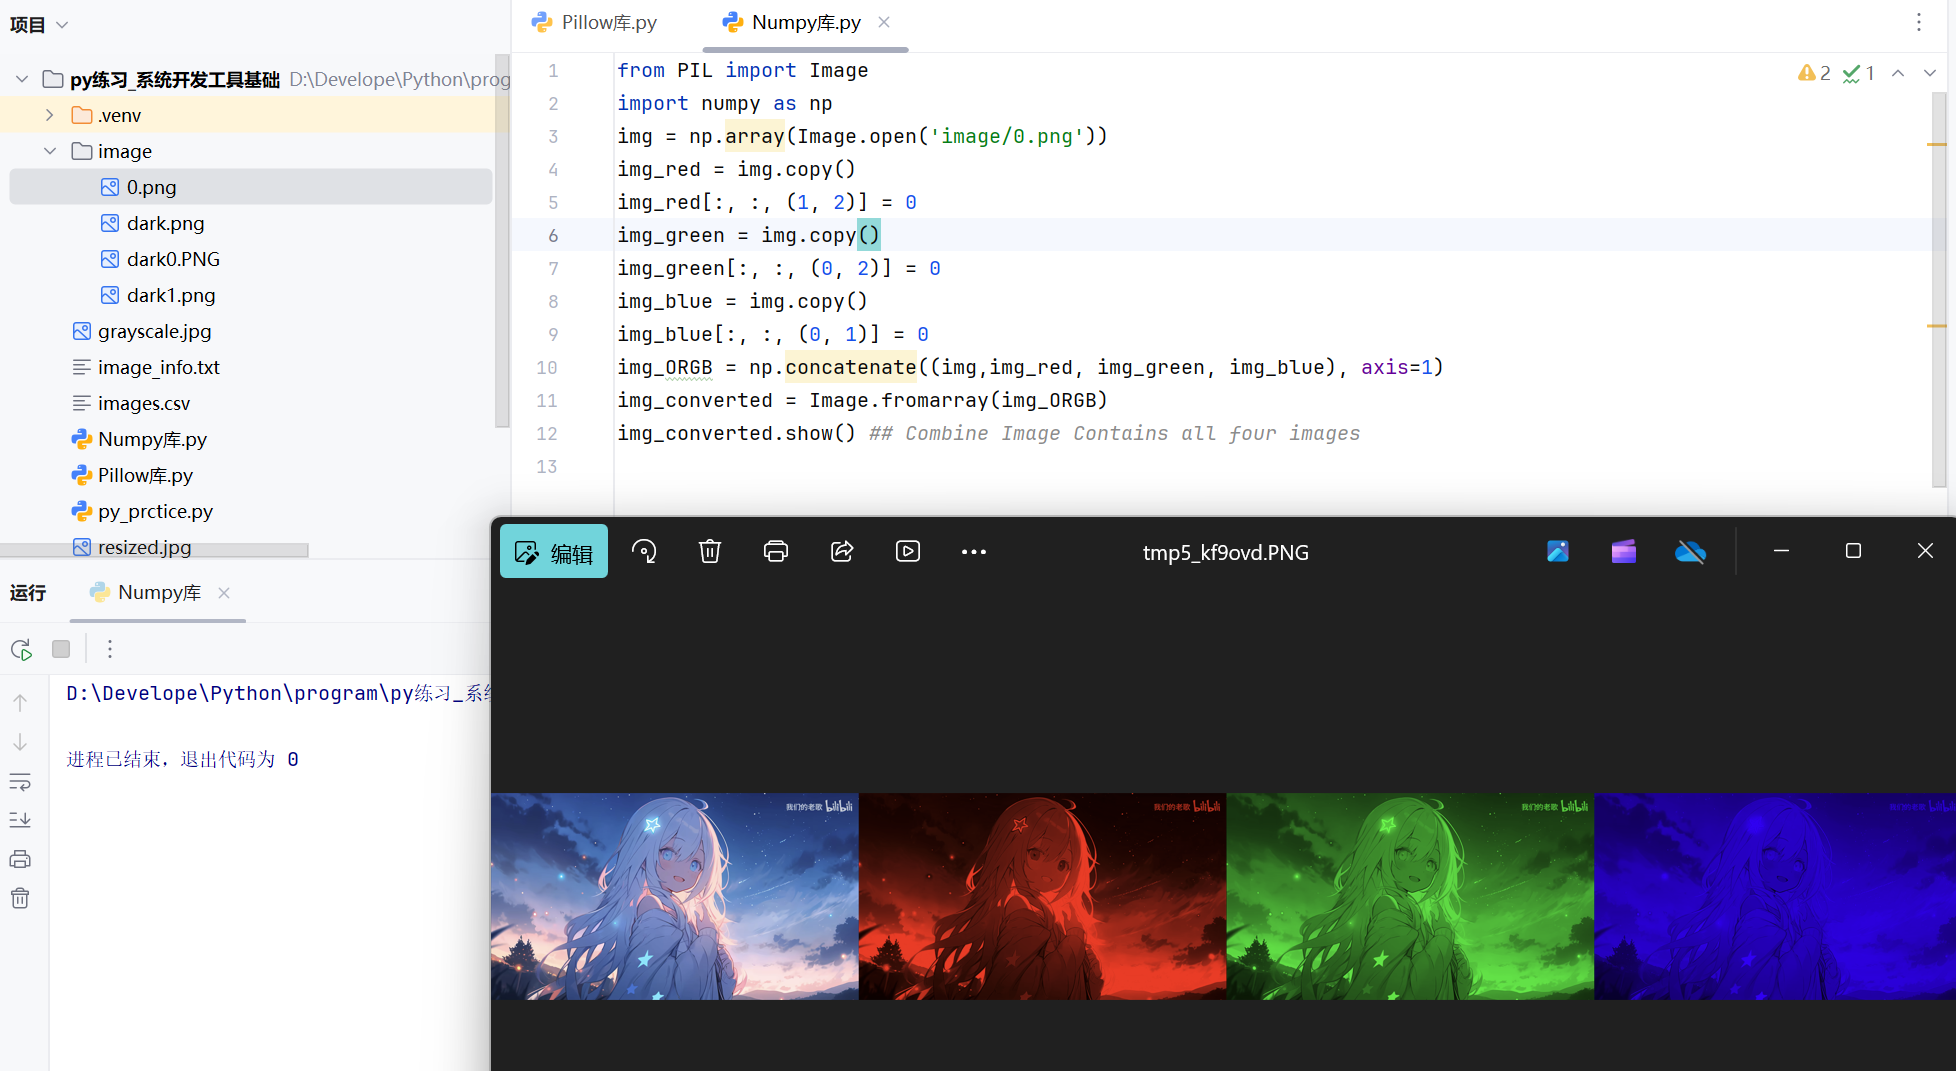
\includegraphics[width=1\textwidth]{image/17.png}
    \caption{实例18}
  \end{figure}
\FloatBarrier

      \begin{figure}[htbp]
    \centering
    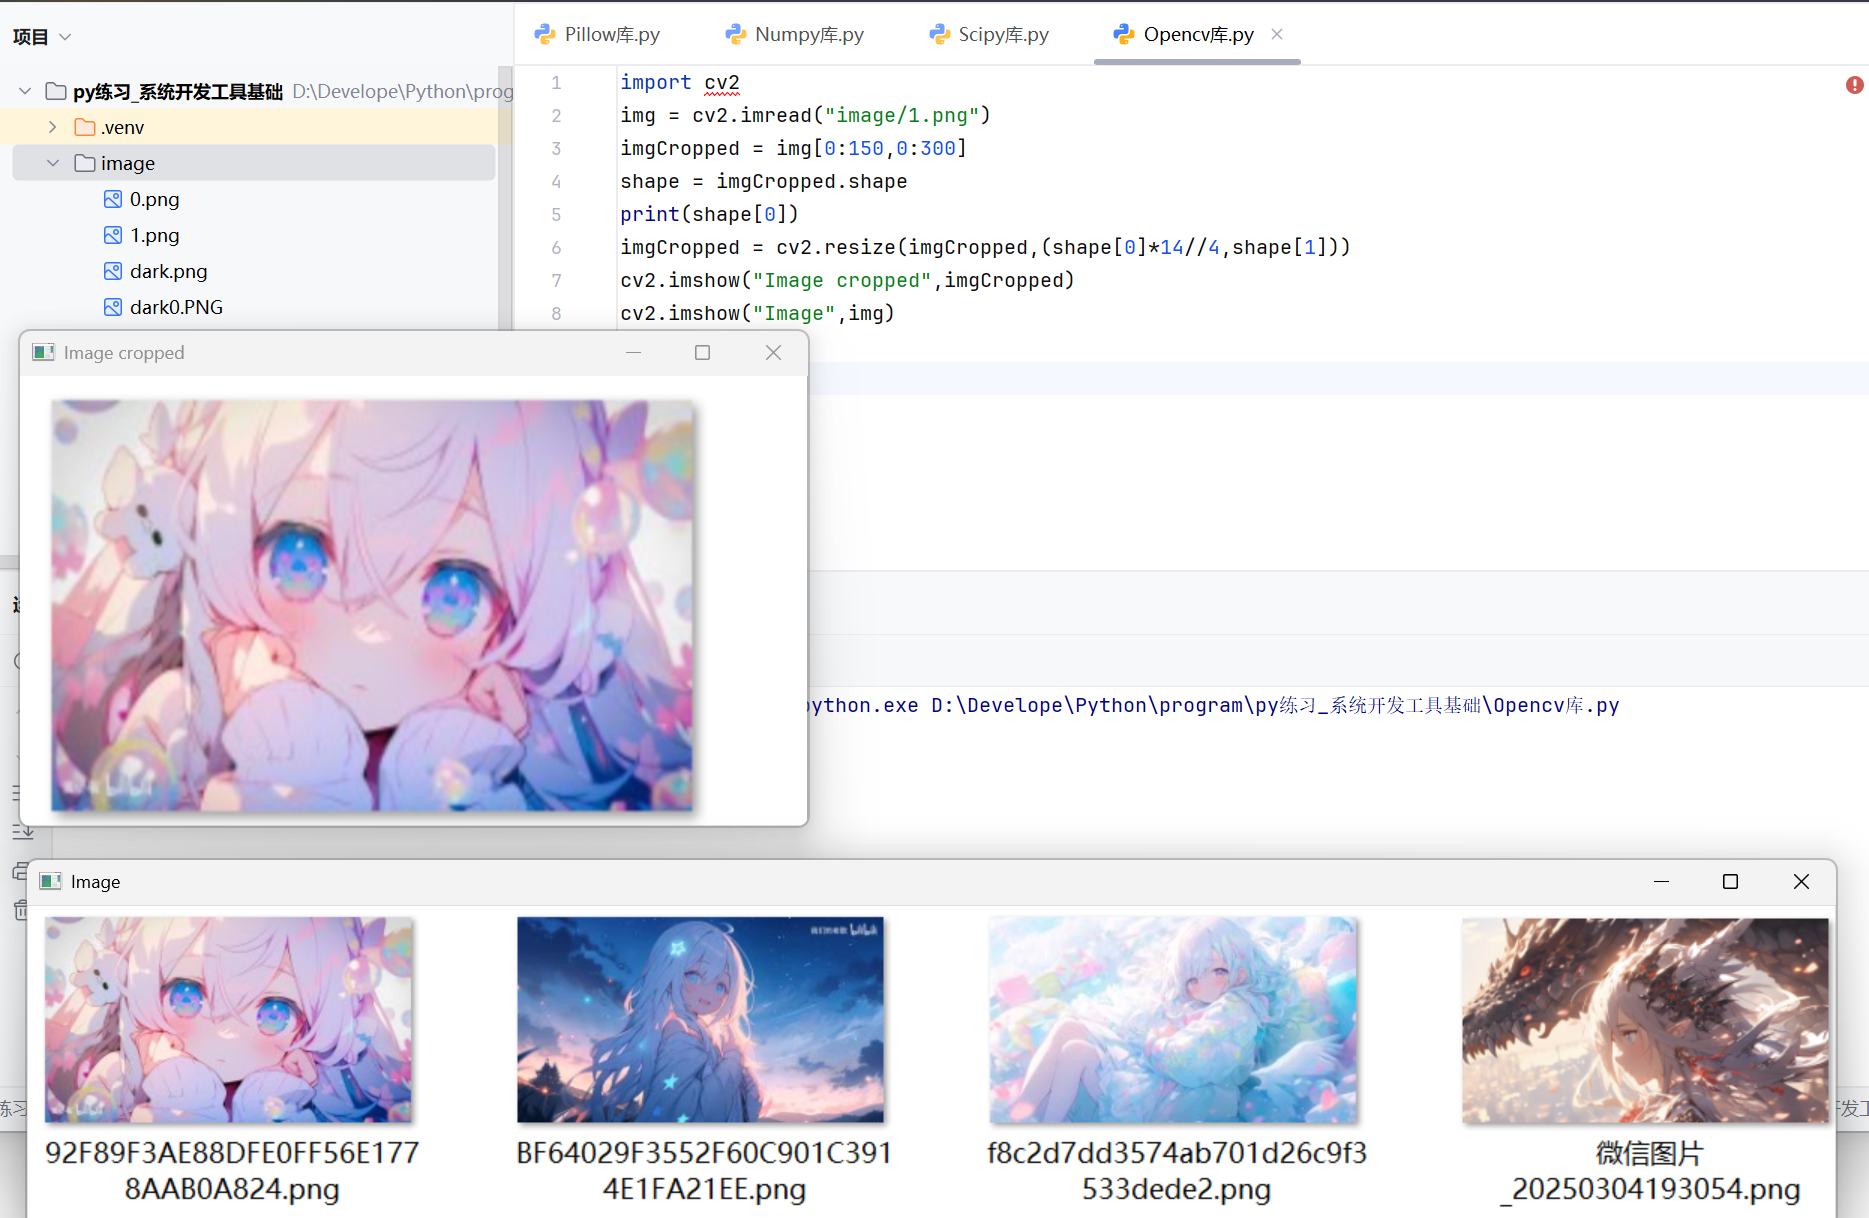
\includegraphics[width=1\textwidth]{image/18.png}
    \caption{实例19}
  \end{figure}
\FloatBarrier

      \begin{figure}[htbp]
    \centering
    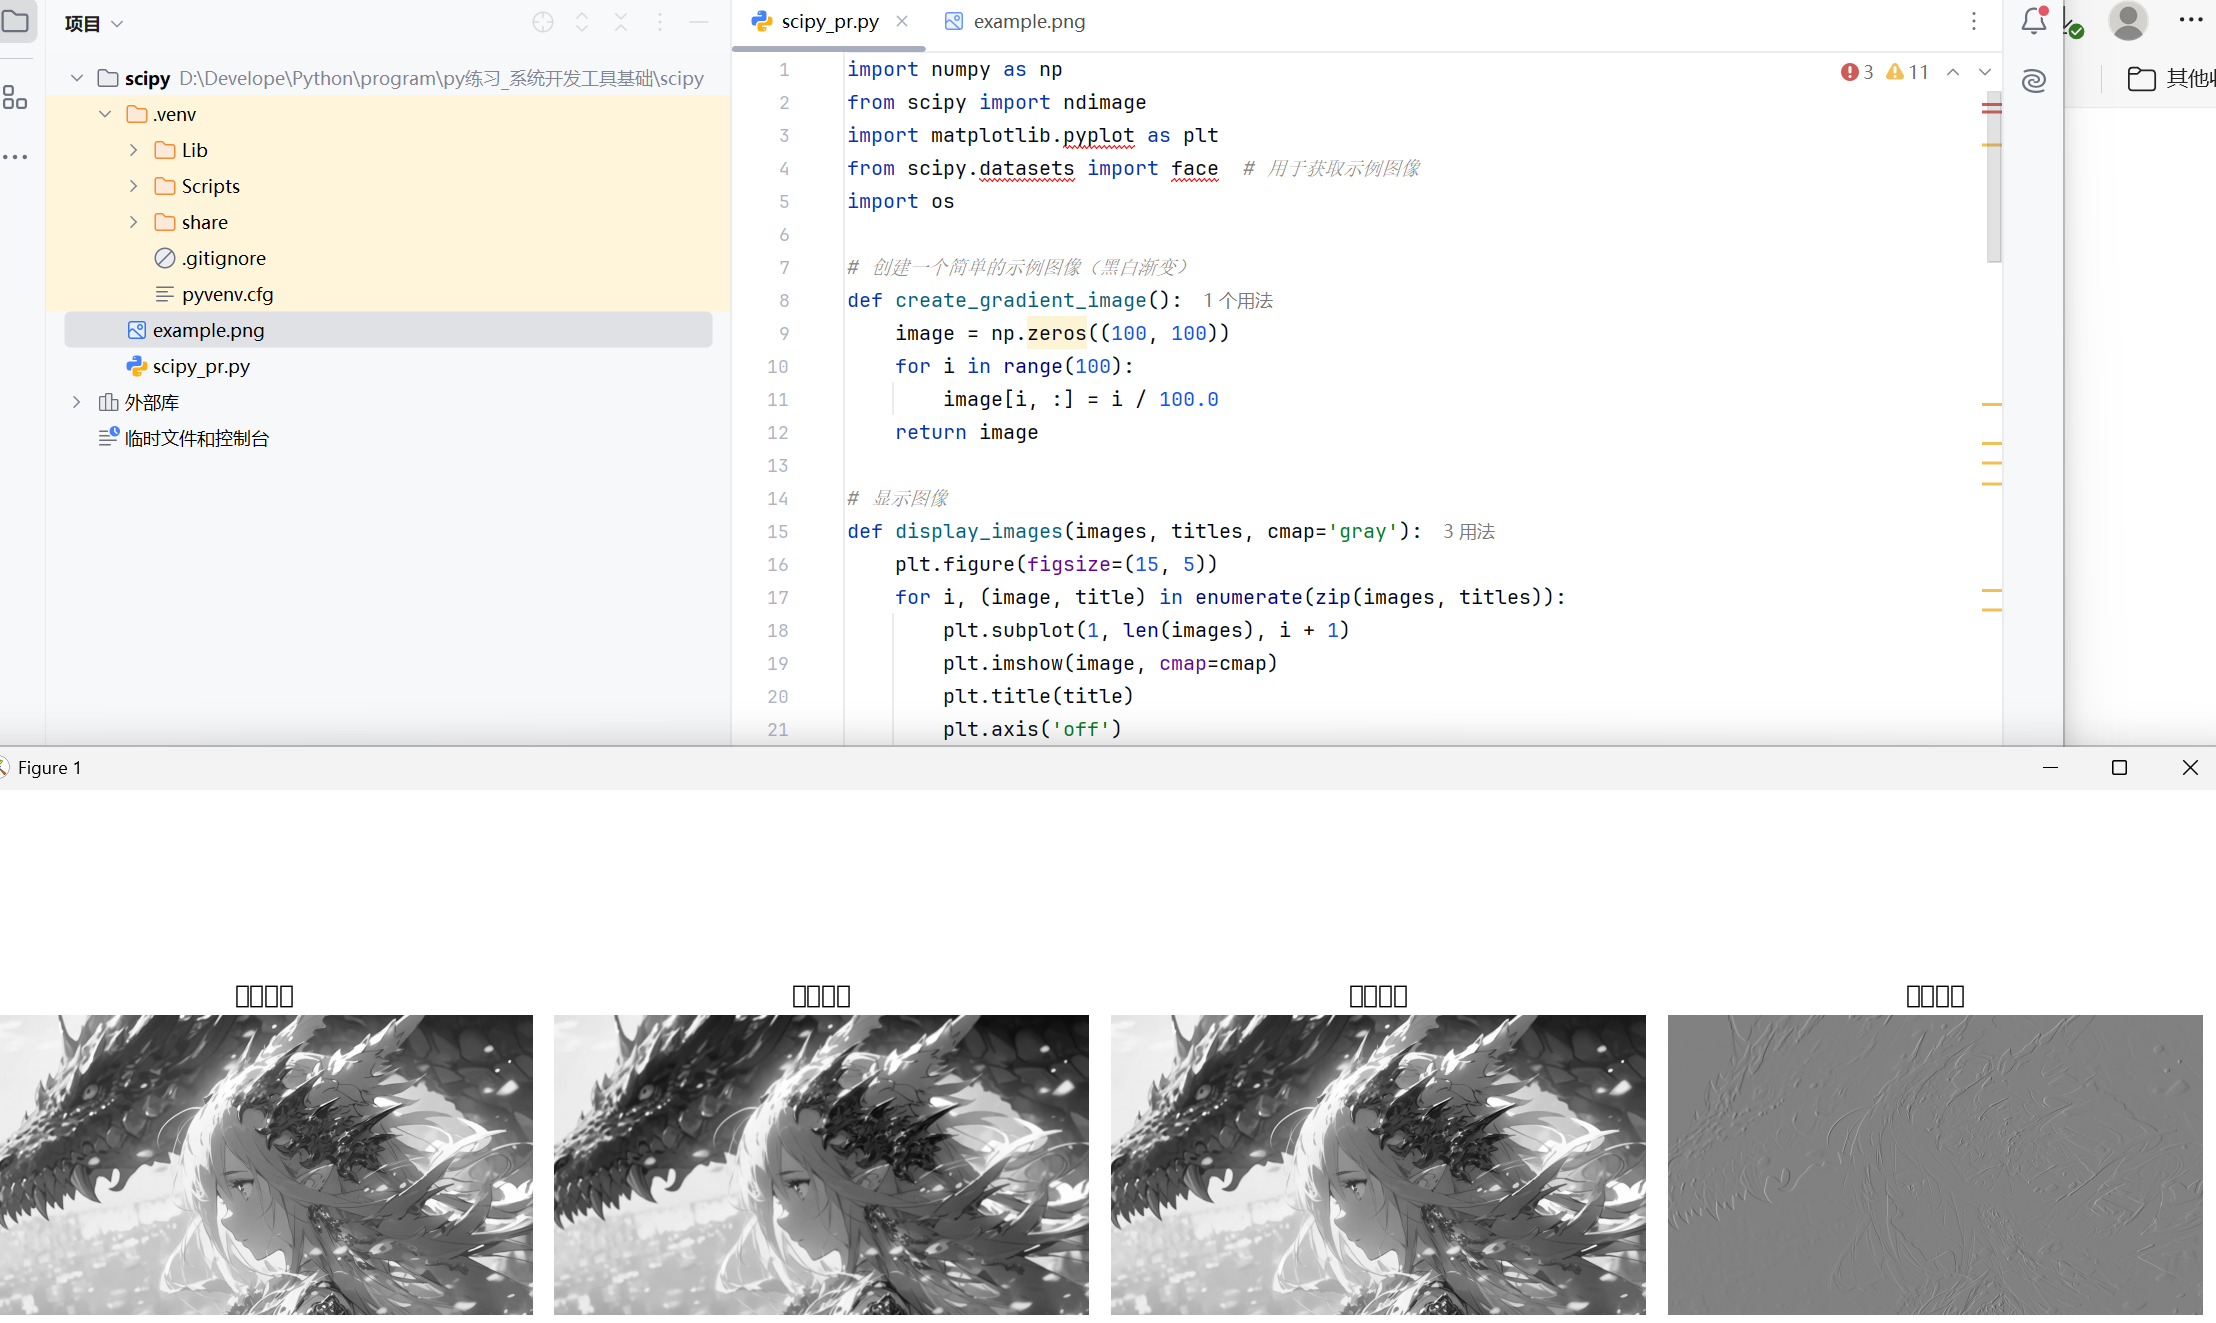
\includegraphics[width=1\textwidth]{image/19.png}
    \caption{实例20}
  \end{figure}
\FloatBarrier
}

\section{解题感悟}

从最初的Shell任务控制到复杂的Python图像处理,从使用tmux进行多任务管理到通过SSH远程操作服务器,
我逐渐认识到了命令行工具与脚本编程在现代开发中具有着重要意义。
而在利用Python的Pillow和OpenCV库处理图像的过程中,我也感受到了自动化与高效开发的魅力。

过程中也遇到不少挑战,比如信号处理的细节、Python中上下文管理器的使用、
以及图像处理中的参数调优等,但通过通过
这些练习,我也有效地巩固了基础知识,同时锻炼了解决问题的能力和代码调试的技巧。

\begin{thebibliography}{99}
\bibitem{} 计算机教育中缺失的一课.命令行环境:\href{https://missing-semester-cn.github.io/2020/command-line/}{https://missing-semester-cn.github.io/2020/command-line/}
\bibitem{} RUNOOB.Python 基础教程:\href{https://www.runoob.com/python/python-tutorial.html}{https://www.runoob.com/python/python-tutorial.htmlxt}
\bibitem{} CSDN.【Python】推荐五个常用的图像处理库:\href{https://blog.csdn.net/sgzqc/article/details/124871774}{https://blog.csdn.net/sgzqc/article/details/124871774}
\bibitem{} CSDN.pycharm虚拟环境的启动,关闭,以及新建虚拟环境:\href{https://blog.csdn.net/qq_29948297/article/details/108354822}{https://blog.csdn.net/qq\_{}29948297/article/details/108354822}
\bibitem{} CSDN.一文详解Pytest单元测试【保姆级教程】.命令行环境:一文详解Pytest单元测试【保姆级教程】:\href{https://blog.csdn.net/fengyuyeguirenenen/article/details/129020897}{https://blog.csdn.net/fengyuyeguirenenen/article/details/129020897}
\end{thebibliography}


\end{document}


